\documentclass{scu-thesis}
\usepackage{vmargin}
\usepackage{multicol}
\setlength\columnsep{20pt}
\setmarginsrb{3 cm}{2.5 cm}{3 cm}{2.5 cm}{1 cm}{1.5 cm}{1 cm}{1.5 cm}
\usepackage{graphicx}	% for including graphics
\renewcommand{\familydefault}{\sfdefault}
\usepackage{multirow}
\usepackage{subcaption}
\usepackage{graphicx}
\usepackage{listings}
\usepackage{color}

\definecolor{mygreen}{rgb}{0,0.6,0}
\definecolor{mygray}{rgb}{0.5,0.5,0.5}
\definecolor{mymauve}{rgb}{0.58,0,0.82}

\lstset{ %
  backgroundcolor=\color{white},   % choose the background color; you must add \usepackage{color} or \usepackage{xcolor}; should come as last argument
  basicstyle=\footnotesize,        % the size of the fonts that are used for the code
  breakatwhitespace=false,         % sets if automatic breaks should only happen at whitespace
  breaklines=true,                 % sets automatic line breaking
  captionpos=b,                    % sets the caption-position to bottom
  commentstyle=\color{mygreen},    % comment style
  deletekeywords={...},            % if you want to delete keywords from the given language
  escapeinside={\%*}{*)},          % if you want to add LaTeX within your code
  extendedchars=true,              % lets you use non-ASCII characters; for 8-bits encodings only, does not work with UTF-8
  frame=single,	                   % adds a frame around the code
  keepspaces=true,                 % keeps spaces in text, useful for keeping indentation of code (possibly needs columns=flexible)
  keywordstyle=\color{blue},       % keyword style
  language=Octave,                 % the language of the code
  morekeywords={*,...},            % if you want to add more keywords to the set
  numbers=left,                    % where to put the line-numbers; possible values are (none, left, right)
  numbersep=5pt,                   % how far the line-numbers are from the code
  numberstyle=\tiny\color{mygray}, % the style that is used for the line-numbers
  rulecolor=\color{black},         % if not set, the frame-color may be changed on line-breaks within not-black text (e.g. comments (green here))
  showspaces=false,                % show spaces everywhere adding particular underscores; it overrides 'showstringspaces'
  showstringspaces=false,          % underline spaces within strings only
  showtabs=false,                  % show tabs within strings adding particular underscores
  stepnumber=2,                    % the step between two line-numbers. If it's 1, each line will be numbered
  stringstyle=\color{mymauve},     % string literal style
  tabsize=2,	                   % sets default tabsize to 2 spaces
  title=\lstname                   % show the filename of files included with \lstinputlisting; also try caption instead of title
}



% \usepackage{amsmath}	% for advanced typesetting of mathematics
% \usepackage{txfonts}	% for using the Times-Roman font
% \usepackage{natbib}	% for better citation styles


% These must be set first ... the rest of the thesis commands rely on them.

\author{Yang Li}
\author{Luis Abraham Millan}
\author{David Blake Tsuzaki}
\title{Portable Reading Assistant Headset for the Visually Impaired}
\department{Department of Computer Engineering}
\department{Department of Electrical Engineering}
\degree{Bachelor of Science in Computer Science and Engineering}
\degree{Bachelor of Science in Electrical Engineering}


% Only bachelor's theses should have multiple authors and/or be from
% multiple departments.  Signatures required:
%
% Bachelor's theses: advisor(s), department chair(s)
% Master's theses: advisor, reader, department chair
% Doctoral theses: doctoral committee (including advisor), department chair

\begin{document}
\frontmatter
\signature{Thesis Advisor}
\signature{Thesis Advisor}
\signature{Department Chair}
\signature{Department Chair}

\maketitle
\begin{abstract}
Most products in the domain of improving the visually impaired ability to process and understand text focus on the direct translation or dictation of text that is in front of a user. Seldom do such product focus on any type of textual understanding that goes beyond literal translation. In this report, we are documenting the implementation of a novel wearable device that allows the visually impaired to have a better understanding of the textual world around them by having a system learn a textual understanding for them and then provide more significant and natural feedback based on a user's semantic queries regarding the text before them.This document includes the requirements, design, use cases, risk tables, workflow and the architecture for the device we developed.
\end{abstract}


\tableofcontents
\listoffigures
\listoftables

\mainmatter
\chapter{Introduction}

\section{Motivation}

Communication is the hallmark of our interactions as humans, occurring across different media, platforms, and entire paradigms. Much of the information we consume on a daily basis is provided by very specialized media, such as a newspaper or a billboard, that caters to only one specific sense, such as vision. This presents a particular challenge for individuals with sensory disabilities. Every day people absorb visual, sonic, and touch information from their surroundings. The visually impaired rely on a heightened sense of sound and touch to obtain information and are hindered from being able to easily obtain data from visual texts, such as posters, newspaper, fliers, etc. This hindrance not only affects their ability to obtain important textual information, such as warning or caution signs, but it also statistically raises the likelihood of unemployment.

\section{Current Solutions}

The Braille alphabet has been one of the most common aids in bridging the gap between textual information for people with visual disabilities. However, Braille presents significant issues around its usability, portability, and adoption. In terms of usability, Braille depends on text being translated and presented on a medium that the user can touch. This assumes the user has some indication of where the text is located, for example, on a sign. Although Braille reading systems exist, these systems are typically very bulky and must be tethered to a personal computer to operate, hindering portability. Most importantly, Braille suffers from a low literacy rate within the visually impaired community because it requires teachers with specialized training, a luxury that is not always available at public schools in the U.S.
	
There are many products on the market that serve as an alternative to Braille. One example is the FingerReader by the MIT Media Lab, an electronic device that dictates the text the user touches in a document. However it can only read 12-point font that the user can physically touch. Another example, the OrCam MyEye, is a dedicated wearable headset that also performs live text dictation and can is marketed as having the capability to read text within the user's reach. However, it is priced at \$2,500 which is outside the price range of many users in this segment. More significantly, its gestural input requires that the user has some visual capability to find the text. Although the FingerReader and OrCam products make significant strides toward usability and effectiveness, they still fall short of being truly practical for most users.

\section{New Solution}

There is a general issues we identified with all the current solutions involve the total cost, usability, and practicality of the system. With this system we seek to address the shortcomings of each, while incorporating their advantages. We have designed an assistive Optical Character Recognition (OCR) system consisting of a portable headset that captures a feed of the user's surroundings, a front-end mobile application that performs live OCR of the text within this feed, and a back-end framework for building a model of textual understanding. This system is capable of reading aloud the key points of the text the user is positioned to “gaze” at and allow the user to manipulate the translation in real-time. As with OrCam, we chose a headset form-factor to serve as the basis for capturing the user's surroundings so that the system's input follows the user's head movement in a natural, unobstructive manner. By using computer vision, we allow the user to focus on text both close as a handheld newspaper and as far as a billboard. With a mobile phone for processing, rather than dedicated hardware, we address another key shortcoming of the current solutions by keeping the cost of the device down and allowing the system to build a model for better dictation in the future. With this system, we hope to address one of the biggest daily challenges of individuals who are visually impaired, a very underserved segment of our society.
\chapter{Requirements}
The Requirements section presents a categorized and itemized list of project requirements. Categories include Functional and Non-functional Requirements and Design Constraints. Functional requirements define what must be done, while non-functional requirements define the manner in which the functional requirements need to be achieved. Both categories have sub-categories, determined by the importance of a given requirement. Design Constraints are similar to non-functional requirements but constrain the solution and not the problem.
\section{Functional Requirements:}
\begin{itemize}
\item Critical
	\begin{itemize}
	\item have sensors to communicate with the user and detect the user's surroundings
	\item communicate with the user through haptic feedback and voice dictation
    \end{itemize}
\item Recommended
	\begin{itemize}
	\item have a learning model to tag specific instances of text and symbols and improve overall recognition
	\end{itemize}
\end{itemize}

\pagebreak

\section{Non-functional Requirements:}
\begin{itemize}
\item Critical
	\begin{itemize}
	\item easy and intuitive to recognize text in the user's environment and dictate it to the user
	\item light and untethered from a large computing system
	\item conform to the Federal Communications Commission guidelines on wearable devices\footnote{https://www.fcc.gov/general/ingestibles-wearables-and-embeddables}
    \end{itemize}
\item Recommended
	\begin{itemize}
	\item maintainable for future usage and/or upgrades
	\end{itemize}
\item Suggested
    \begin{itemize}
	\item generally aesthetically pleasing so that it does not draw too much attention from the user's surroundings
	\end{itemize}
\end{itemize}

\section{Design Constraints}
\begin{itemize}
\item The main device is a wearable headset whose hardware is self-contained
\item The main device's main communication with the outside world is through a smartphone
\item The main device communicates primarily through sound and touch, and not through vision
\end{itemize}

\chapter{Use Cases}
The Use Cases section defines specifics regarding the main, expected interactions between users and the system.

Figure~\ref{useCase} shows the list of use cases that we would like the final product to have, due to time constraints we only implemented the "Reading" use case.

\begin{figure}
	
	\centering
	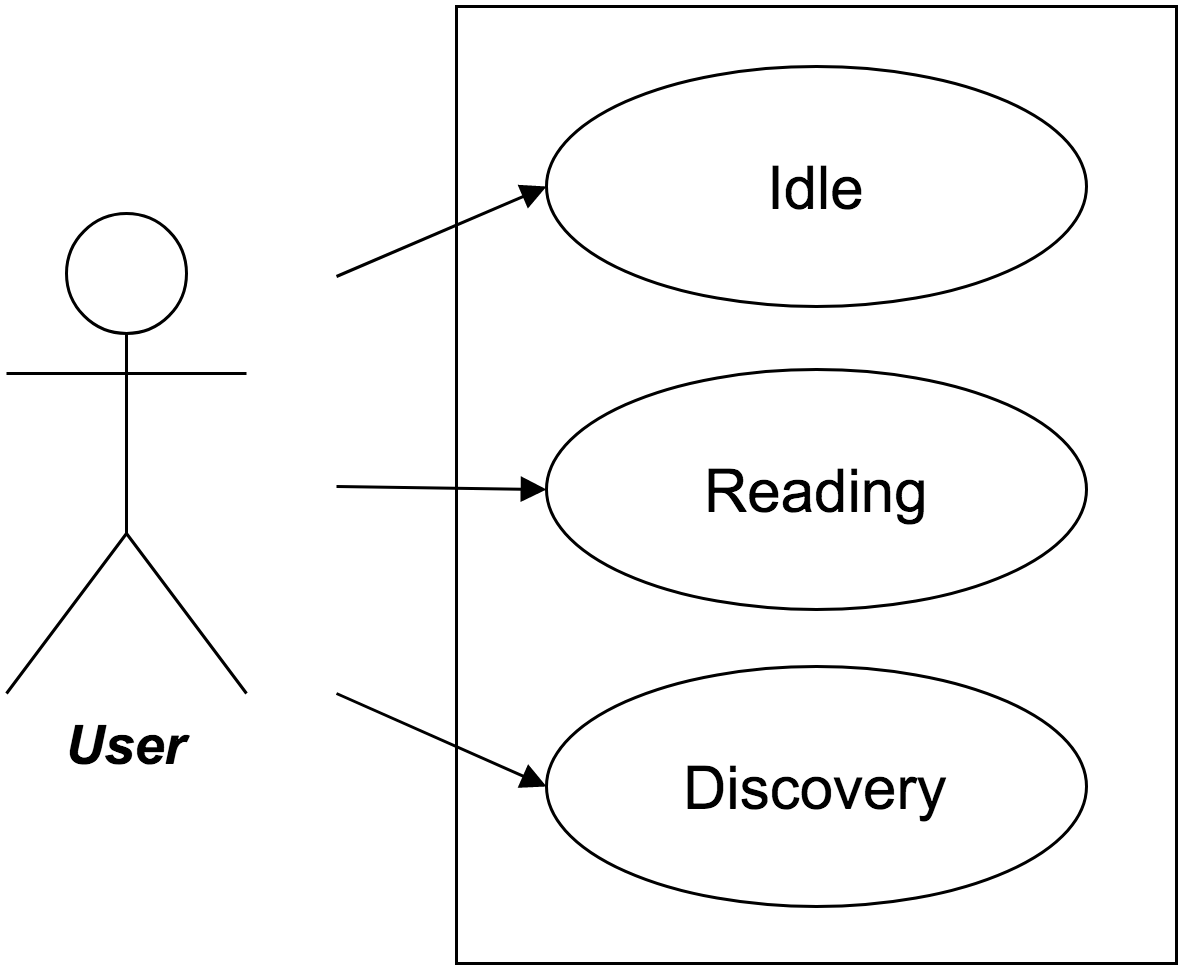
\includegraphics[scale = 0.15]{useCase.png}
    
    \caption{Use Cases}
    \label{useCase}
\end{figure}

\pagebreak

\subsubsection{Idle}
\begin{description}
\item [Goal] Put the device to sleep to preserve power.
\item [Actor] User
\item [Preconditions] Device must be turned on
\item [Steps] User set the device to idle
\item [Postconditions] Disconnect connection to headset and server
\item [Exceptions] N/A
\end{description}


\subsubsection{Reading}
\begin{description}
\item [Goal] Identify and obtain large amount of text and provide feedback to user
\item [Actor] User
\item [Preconditions] Device must be turned on and set to Reading Mode
\item [Steps] User stare at the document he will to know and order the device to capture the image
\item [Postconditions] Audio feedback send to user
\item [Exceptions] Unstable input, such that the motion of the headset is outside the threshold
\end{description}


\vspace{5mm}


\subsubsection{Discovery}
\begin{description}
\item [Goal] Inform the user about potential point of interest around him or her
\item [Actor] User
\item [Preconditions] Device must be turned on and set to Discovery Mode
\item [Steps] User need to move his or her head around to capture the surrounding
\item [Postconditions] Audio feedback send to user
\item [Exceptions] Unstable input, such that the motion of the headset is outside the threshold
\end{description}
\chapter{Activity Diagram}
Figure~\ref{activityDiagram} is the activity diagram that shows the flow of actions of the user.
During each decision stage, the system will prompt the user for actions.


\begin{figure}
	\centering
    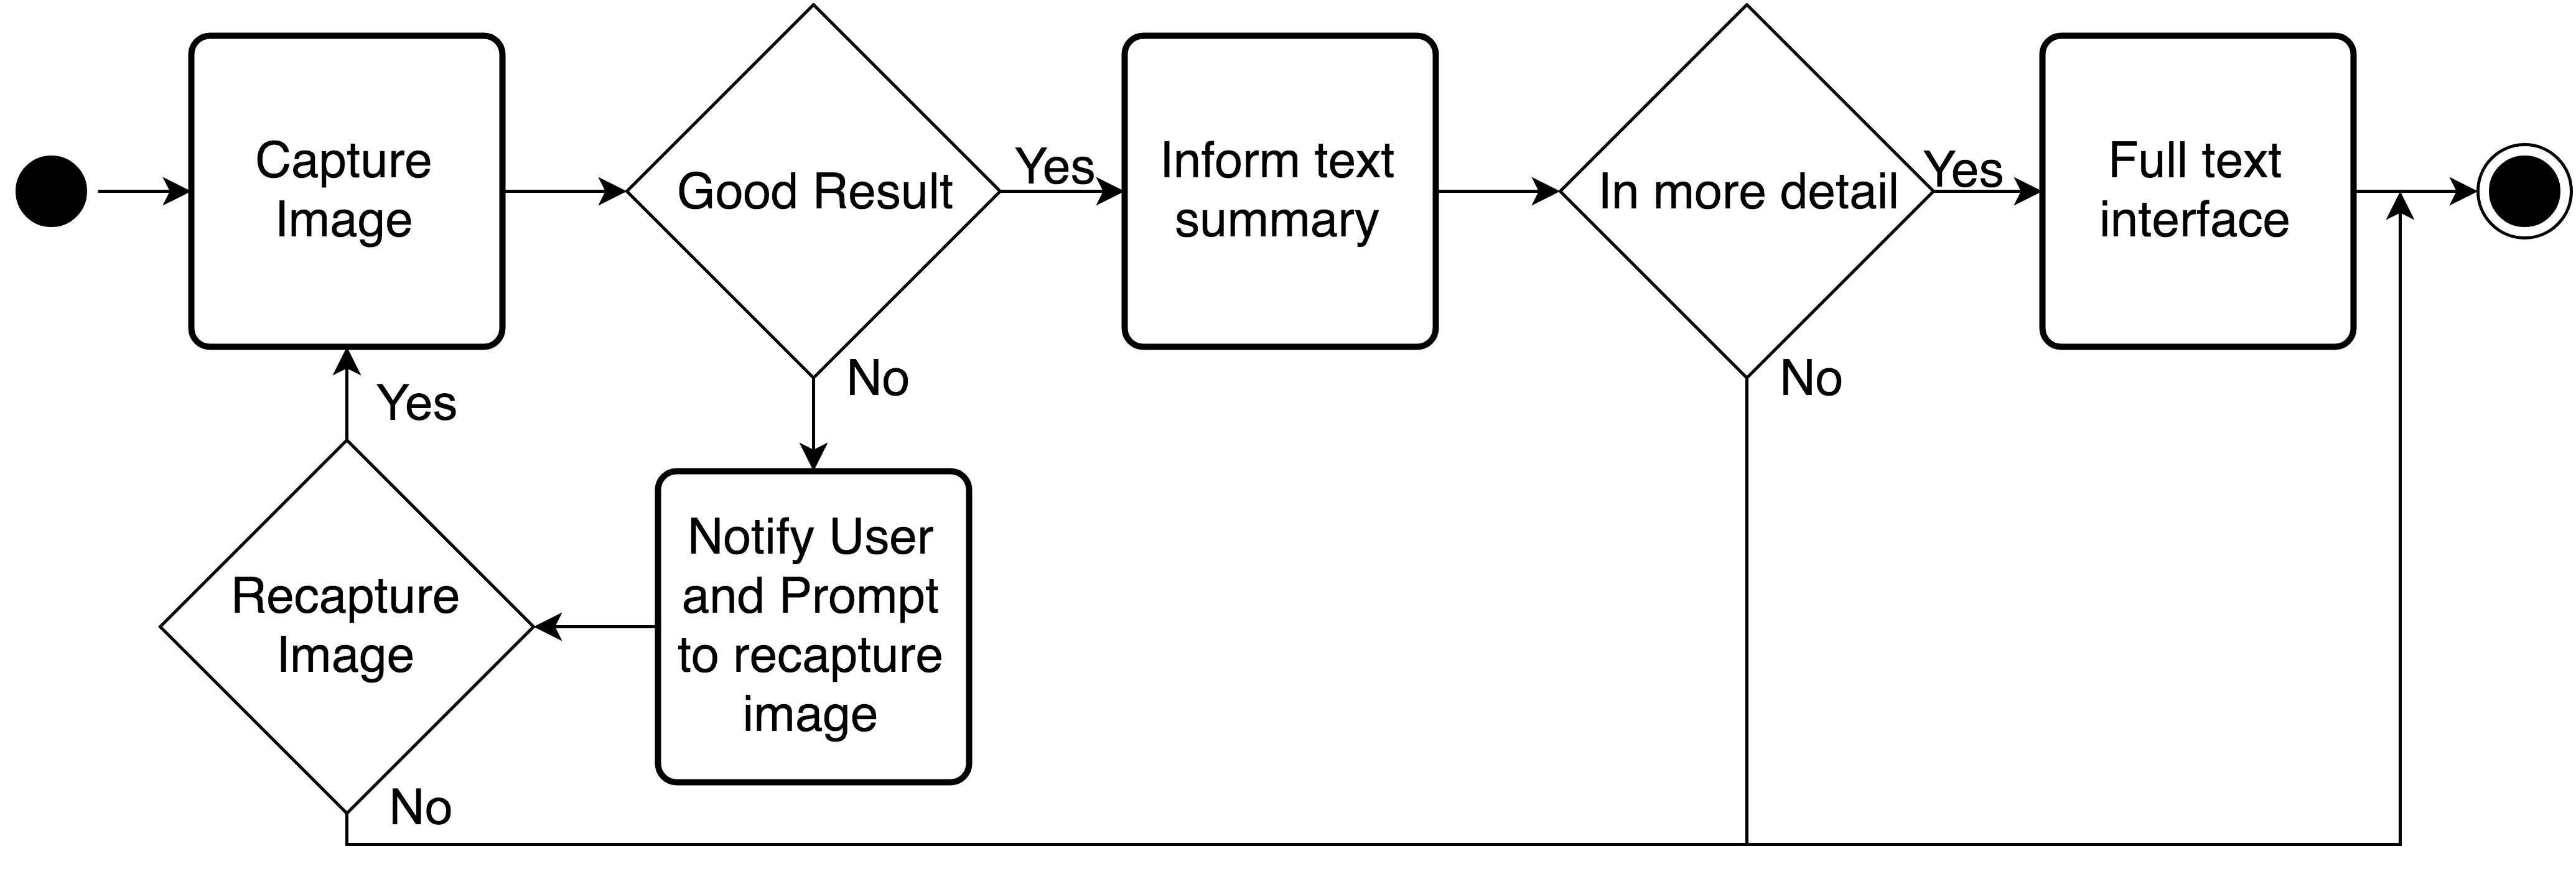
\includegraphics[scale = 0.26]{Activity_H.png}%{activityDiagram.png}
    
    \caption{Activity Diagram}
	\label{activityDiagram}
\end{figure}
%\chapter{Conceptual Model}
The following is the conceptual model of the physical product
\chapter{Technologies Used}



\section{Tesseract Optical Character Recognition Engine:}
An open source OCR engine licensed under Apache License, Version 2.0\footnotemark. It is one of the most accurate open source OCR engines currently available.


\section{TensorFlow:}
	An open source library of programing functions for machine learning. Licensed under Apache License, Version 2.0\footnotemark[\value{footnote}].

\footnotetext{https://www.apache.org/licenses/LICENSE-2.0.txt}

\section{OpenCV:}
An open source library of programing functions mainly aimed at real-time computer vision. Licensed under BSD license\footnotemark.


\section{NumPy:}
	An extension (numerical and scientific library) to the Python programming language, it adds support for large, multidimensional arrays and matrices. Licensed under BSD-new license\footnotemark[\value{footnote}].


\section{scikit-learn:}
	A free machine learning library for Python programming language, designed to interoperate with NumPy and SciPy. Licensed under BSD license\footnotemark[\value{footnote}]. 


%\section{scikit-image:}
%	An image processing library for Python programming language, designed to interoperate with NumPy and SciPy. Licensed under BSD license\footnotemark[\value{footnote}].

\footnotetext{https://en.wikipedia.org/wiki/BSD\_licenses}
\chapter{Architecture}

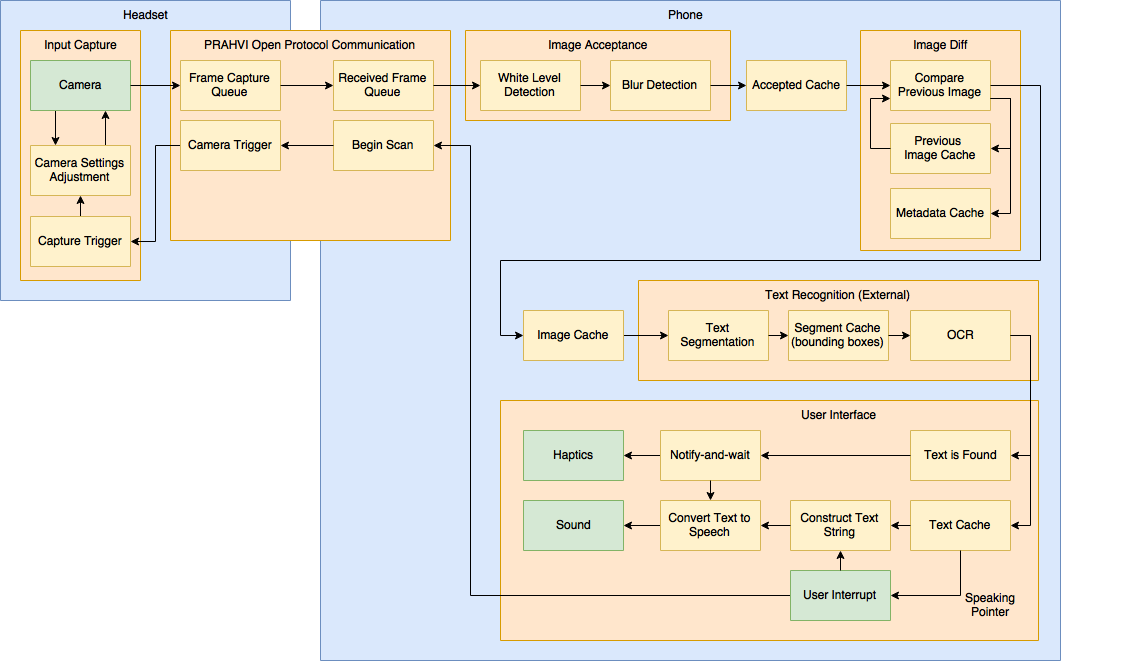
\includegraphics[scale = 0.4]{PRAHVI-Block.png}

\section{Activity Diagram}
Figure~\ref{activityDiagram} is the high level data-flow architecture of the system that shows the flow of actions of the user. Input is first received by the system to begin capturing an image of the user's immediate gaze, or view, in front of them. The system then evaluates the image and notifies the user if the image needs to be recaptured because it is too blurry or the text is illegible. If the image passes this evaluation, the system then translates the image into text and generates a summary for the user. This summary is then read aloud to the user. If the user takes no action at this point, the system proceeds to reading the entire text article. This architecture was chosen because there are constant inputs received by the system, and the inputs in general goes through the same route within the system. The data-flow architecture also has build-in concurrency, which can speeds up the process, especially the platform in which the product is embedded.

\begin{figure}
	\centering
    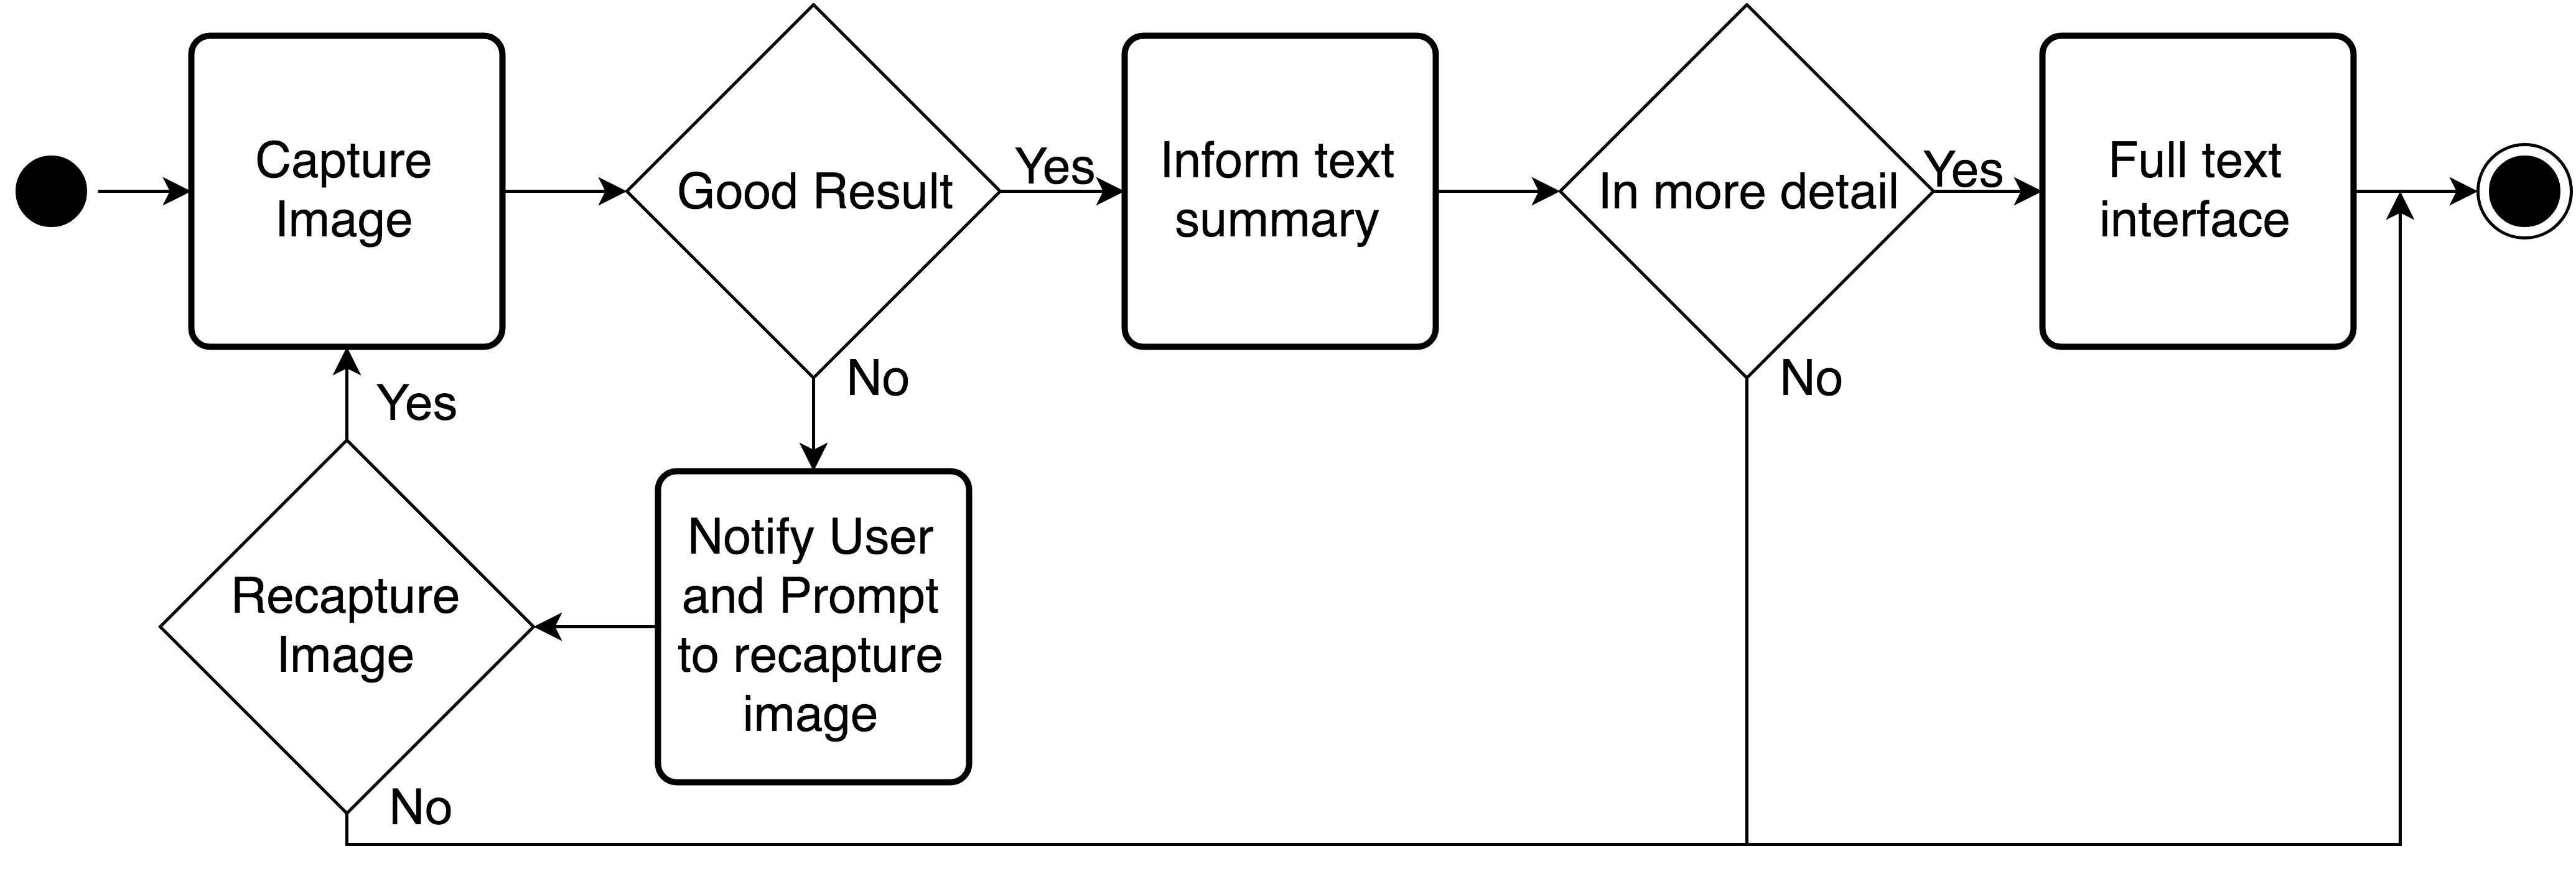
\includegraphics[scale = 0.105]{Activity_H.png}%{activityDiagram.png}
    
    \caption{High Level View}
	\label{activityDiagram}
\end{figure}

\section{Hardware}
The most visible component of PRAHVI is its wearable headset device that attaches to a typical pair of glasses or can be manufactured as a single assembly. The headset (shown in appendix \ref{headsetPic}) is comprised of a Raspberry Pi Zero board coupled with a standard Raspberry Pi Camera. The Raspberry Pi Zero was chosen for its low power consumption, small footprint, and its UNIX-based operating system allows for wide application flexibility. This means that the Raspberry Pi Zero allows us to cut down on the device's size and weight while creating an extensible application platform. Its main shortcoming, processor speed, is mitigated by the fact we use a smartphone and external server to process the images. The Raspberry Pi Camera is a module comprised of a breakout board and a 5.0 megapixel smartphone camera. The cable used to connect the camera to the Raspberry Pi Zero is a standard accessory cable used by many third-party accessories. Together, the Raspberry Pi Zero and the camera module can be acquired for less than \$60, helping to bring the cost of a single device down for users. The modular nature of these parts allows for future expansion and easy repairs for the user and for other developers. 

When the device is connected to the user's smartphone and the accompanying app is opened, PRAHVI powers up and immediately begins communicating with the smartphone. Once the initial setup is completed, the headset waits for a trigger from the user to begin capturing images of the user's surroundings. Once this is triggered, the camera begins capturing a set of images which are added to a frame capture queue and used to adjust the camera settings, such as white balance and exposure, to achieve an optimal capture. An image sample is then served over the bridge created using the PRAHVI Open Protocol back to the smartphone. PRAHVI Open Protocol, or "POP," is a socket-oriented connection protocol based on the open source Bonjour networking standard.\footnote{https://developer.apple.com/bonjour/} Although the protocol is implemented for iOS and Python for this product, the protocol can be implemented on any platform or system that supports network sockets. These technologies and systems were ultimately employed to make using PRAHVI, from the moment the user connects the device, to the point the user requests a translation, as seamless and intuitive as possible from an ergonomics standpoint.

\begin{figure}
	\centering
	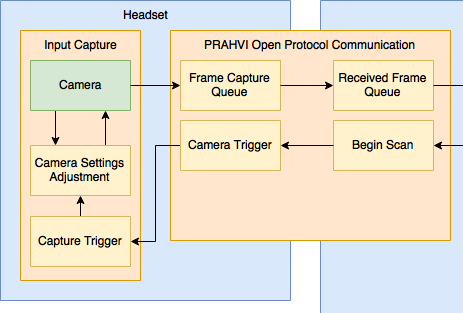
\includegraphics[scale = 0.6]{PRAHVI-HEADSET}
	\caption{Hardware Diagram}
	\label{headsetDiagram}
\end{figure}

\section{User Interface}
The user interface of PRAHVI is designed to operate entirely using haptic feedback and voice to simplify interaction and make text translation seamless. For this product, an app was written on the iOS platform to communicate with the headset device. The app (shown in \ref{uipicture}) is mainly comprised of a gesture pad that spans three fourths of the entire surface of the phone screen. Once the user connects the headset and opens the app, PRAHVI immediately connects to the app to set up the POP connection. When the user double taps the gesture area, the device begins scanning the environment, adjusting the camera parameters to find a set point that produces clear, usable images. From this queue, an image is selected using image acceptance algorithms and sent to the backend for translation. Once the translation is complete, the app stores the translated text into a cache and signals to the user a quick summary (see Text Summarization section for more information) of the text before proceeding with a full translation. Swiping the gesture area allows the user to navigate the text in realtime, with the smartphone providing haptic feedback. The user primarily interacts with the app to begin translation, proceed from the summary to the full translation, and navigate the translation. By using sound and touch as the primary modes of communication for the user interface, much of the interface could actually be removed, simplifying the experience for users.

\begin{figure}
	\centering
	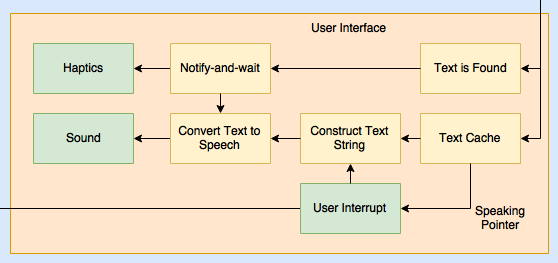
\includegraphics[scale = 0.6]{PRAHVI-UI.png}
	\caption{User Interface Diagram}
	\label{uiDiagram}
\end{figure}

\section{Backend}
The backend of PRAHVI is a flask web application. It exposes all the functionality related to the computer vision, optical character recognition, and text summary into a an easy web interface for our iPhone application to use.

The interface of the backend is a simple set of HTTP endpoints which are summarized as follows:

\begin{table}[]
\centering
\caption{PRAHVI API Endpoints}
\label{PRAHVI_API_endpoints}
\begin{tabular}{|l|l|l|l|l|}
\hline
\multicolumn{1}{|c|}{\textbf{Endpoint}} & \multicolumn{1}{c|}{\textbf{Input}}                                                   & \multicolumn{1}{c|}{\textbf{Output}}                                                                       & \multicolumn{1}{c|}{\textbf{\begin{tabular}[c]{@{}c@{}}HTTP\\ METHOD\end{tabular}}} & \multicolumn{1}{c|}{\textbf{Description}}                                                                                        \\ \hline
/api/v1/image/ocr3                      & File: Image                                                                           & \begin{tabular}[c]{@{}l@{}}JSON: \\ \{ result:\\    string \}\end{tabular}                                 & POST                                                                                & \begin{tabular}[c]{@{}l@{}}PRAHVI's image to text\\ algorithm using tesseract 3\end{tabular}                                     \\ \hline
/api/v1/image/ocr4                      & File: Image                                                                           & \begin{tabular}[c]{@{}l@{}}JSON: \\ \{ result:\\    string \}\end{tabular}                                 & POST                                                                                & \begin{tabular}[c]{@{}l@{}}PRAHVI's image to text\\ algorithm using tesseract 4\end{tabular}                                     \\ \hline
/api/v1/text/tfidf                      & String                                                                                & \begin{tabular}[c]{@{}l@{}}JSON:\\ \{result: \\    \{ term:\\       score, \\       ... \} \}\end{tabular} & POST                                                                                & \begin{tabular}[c]{@{}l@{}}Takes in a document string \\ and outputs the scores of \\ all the terms in the document\end{tabular} \\ \hline
/api/v1/text/compare                    & \begin{tabular}[c]{@{}l@{}}JSON: \\ \{ text1: string,\\ text2: string \}\end{tabular} & \begin{tabular}[c]{@{}l@{}}JSON:\\ \{ result: \\    int{[}0, 1{]} \}\end{tabular}                          & POST                                                                                & \begin{tabular}[c]{@{}l@{}}Returns a score of how\\ similar the documents are\end{tabular}                                       \\ \hline
\end{tabular}
\end{table}



\begin{itemize}

\item Originally, all of the functionality listed above was implemented within the iPhone application, however due to the limited compute resources of the iPhone, PRAHVI's requirements were not being met. Image to text translation on average would take half a min, and the iPhone architecture was mangling some of the text results. For these reasons, these functionalities have been moved the backend end hosted on a server allows for a faster processing time as noted in our test bench. The server is a linux machine running an Intel(R) Core(TM) i7-4900MQ CPU @ 2.80GHz multi-core processor.

\end{itemize}

\section{System Flow}
Once the camera captures the image and sends the image to the smart phone, the image will pass through the pre-processing stage to detect whether the image will be processed or not, based on the blurriness of the image and the similarity of the current image and the previous image (see Image Pre-processing for more information). Once the image has passed the pre-processing stage, it is also processed for text, which is stored in the smart phone. Access to text is by string, and different lines are separated by the new line character that is the same as the document captured. The text is then output as audio feedback as decided by the user (see Figure ).



\section{Text Extraction}

\subsection{Image Pre-processing}
When the smart phone application receives the image, the image is then passed through 2 filters. The first filter detects the blurriness of the image. If the image is blurred, the phone will reject the image because it is hard to extract useful information from a blurred imaged. If the image passed the blurriness test, it will then be used to compare to the previous detected image for similarity. If the image is similar (or the same), the image will also be rejected, because the information from the same document is stored in the device from the previous capture. These 2 filters help to improve the efficiency of the system and save time waited by the user.

\subsubsection{Blurriness Test}

To test for blurriness, variance of Laplacian \cite{PechPacheco} is used. The image is treated as a 2-dimensional matrix (after grayscaled), and convolve it with the 3x3 Laplacian kernel (see Figure~\ref{laplacianKernel}). The variance of Laplacian is the variance of the response. The variance of Laplacian of the image is then compared to a threshold value (the threshold value used for this system is 50). If the variance of Laplacian of the image is lower than the threshold, then the image is blurred, otherwise, it is not.
\begin{figure}
	\centering
    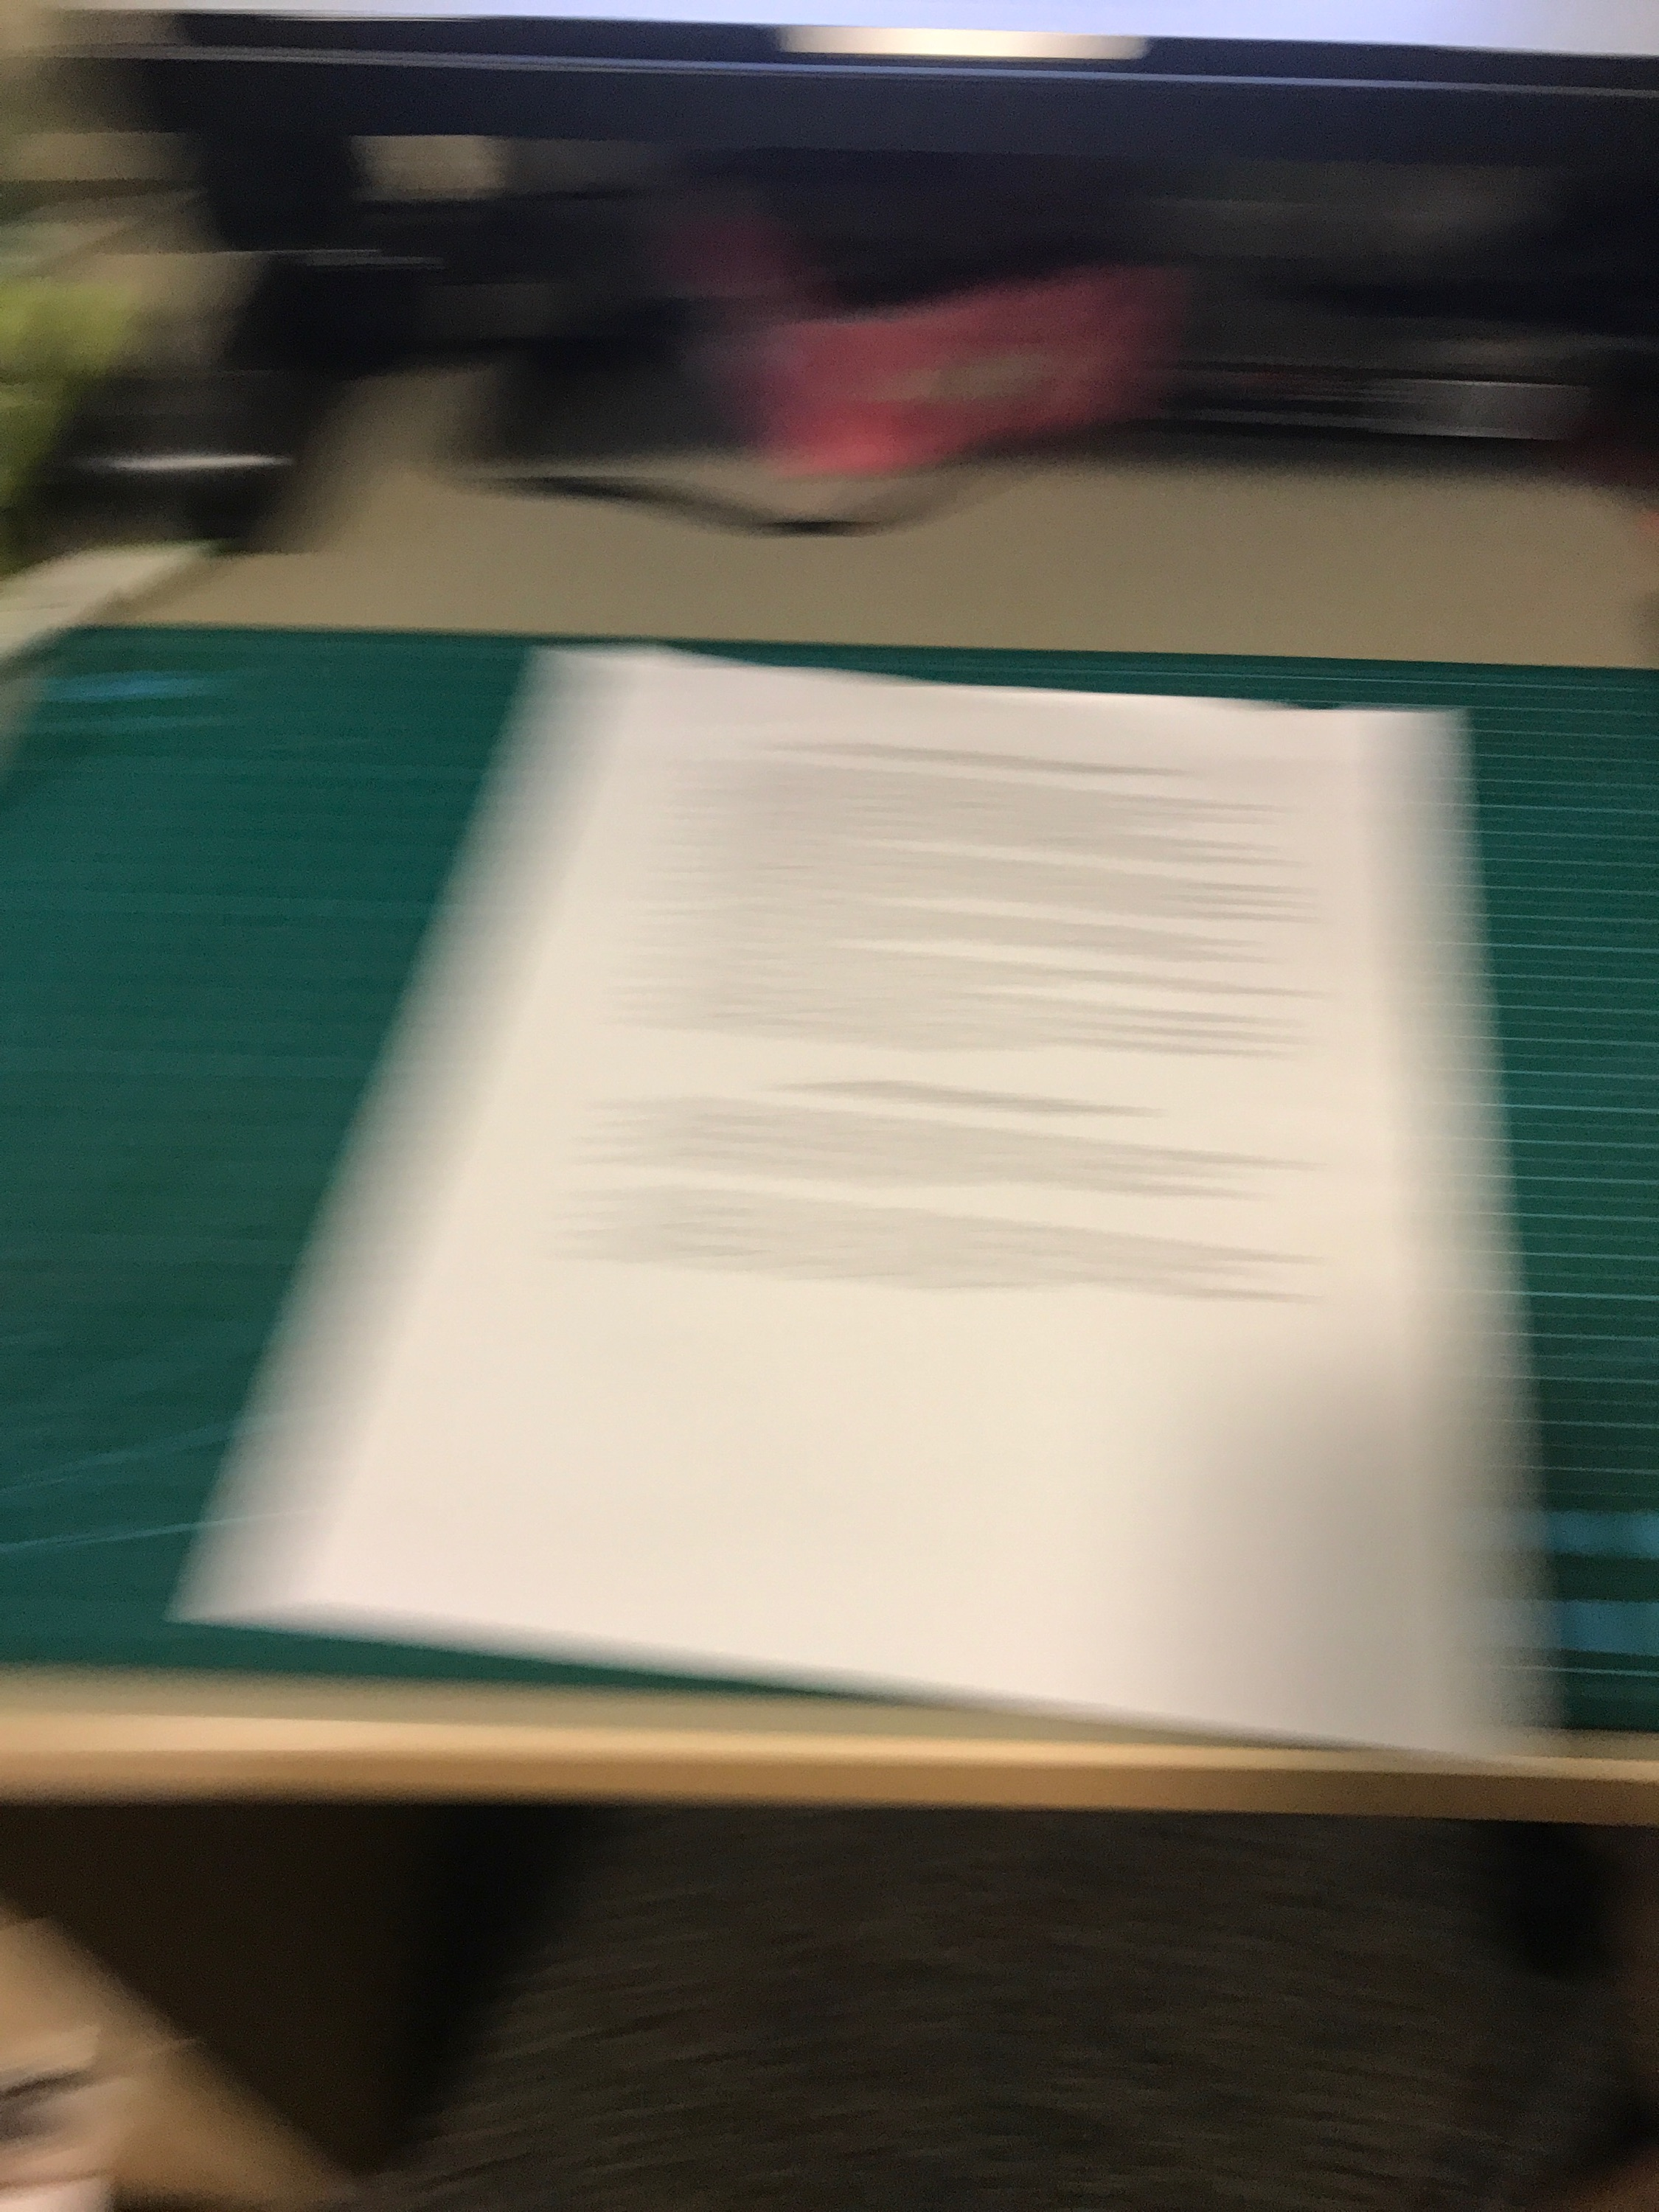
\includegraphics[scale = 0.075]{blur.jpg}
    
    \caption{Blurred image}
	\label{blurredImage}
\end{figure}

\begin{figure}
	\centering
    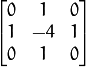
\includegraphics[scale = 0.5]{laplacian_kernel.png}
    
    \caption{The Laplacian kernel}
	\label{laplacianKernel}
\end{figure}

\subsubsection{Similarity Test}
The similarity test uses the accelerated-KAZE (AKAZE) local features matching \cite{akaze}.~The AKAZE local features matching returns a list of matches between the two images. We consider the two image is similar if the number of good matches is above the threshold (the threshold value used for this system is 1000), then the images is said to be similar. In other words, if the two images have the numbers of good matches that is greater than the threshold value, it is said to be similar.

\begin{figure}
  \begin{subfigure}{\linewidth}
	  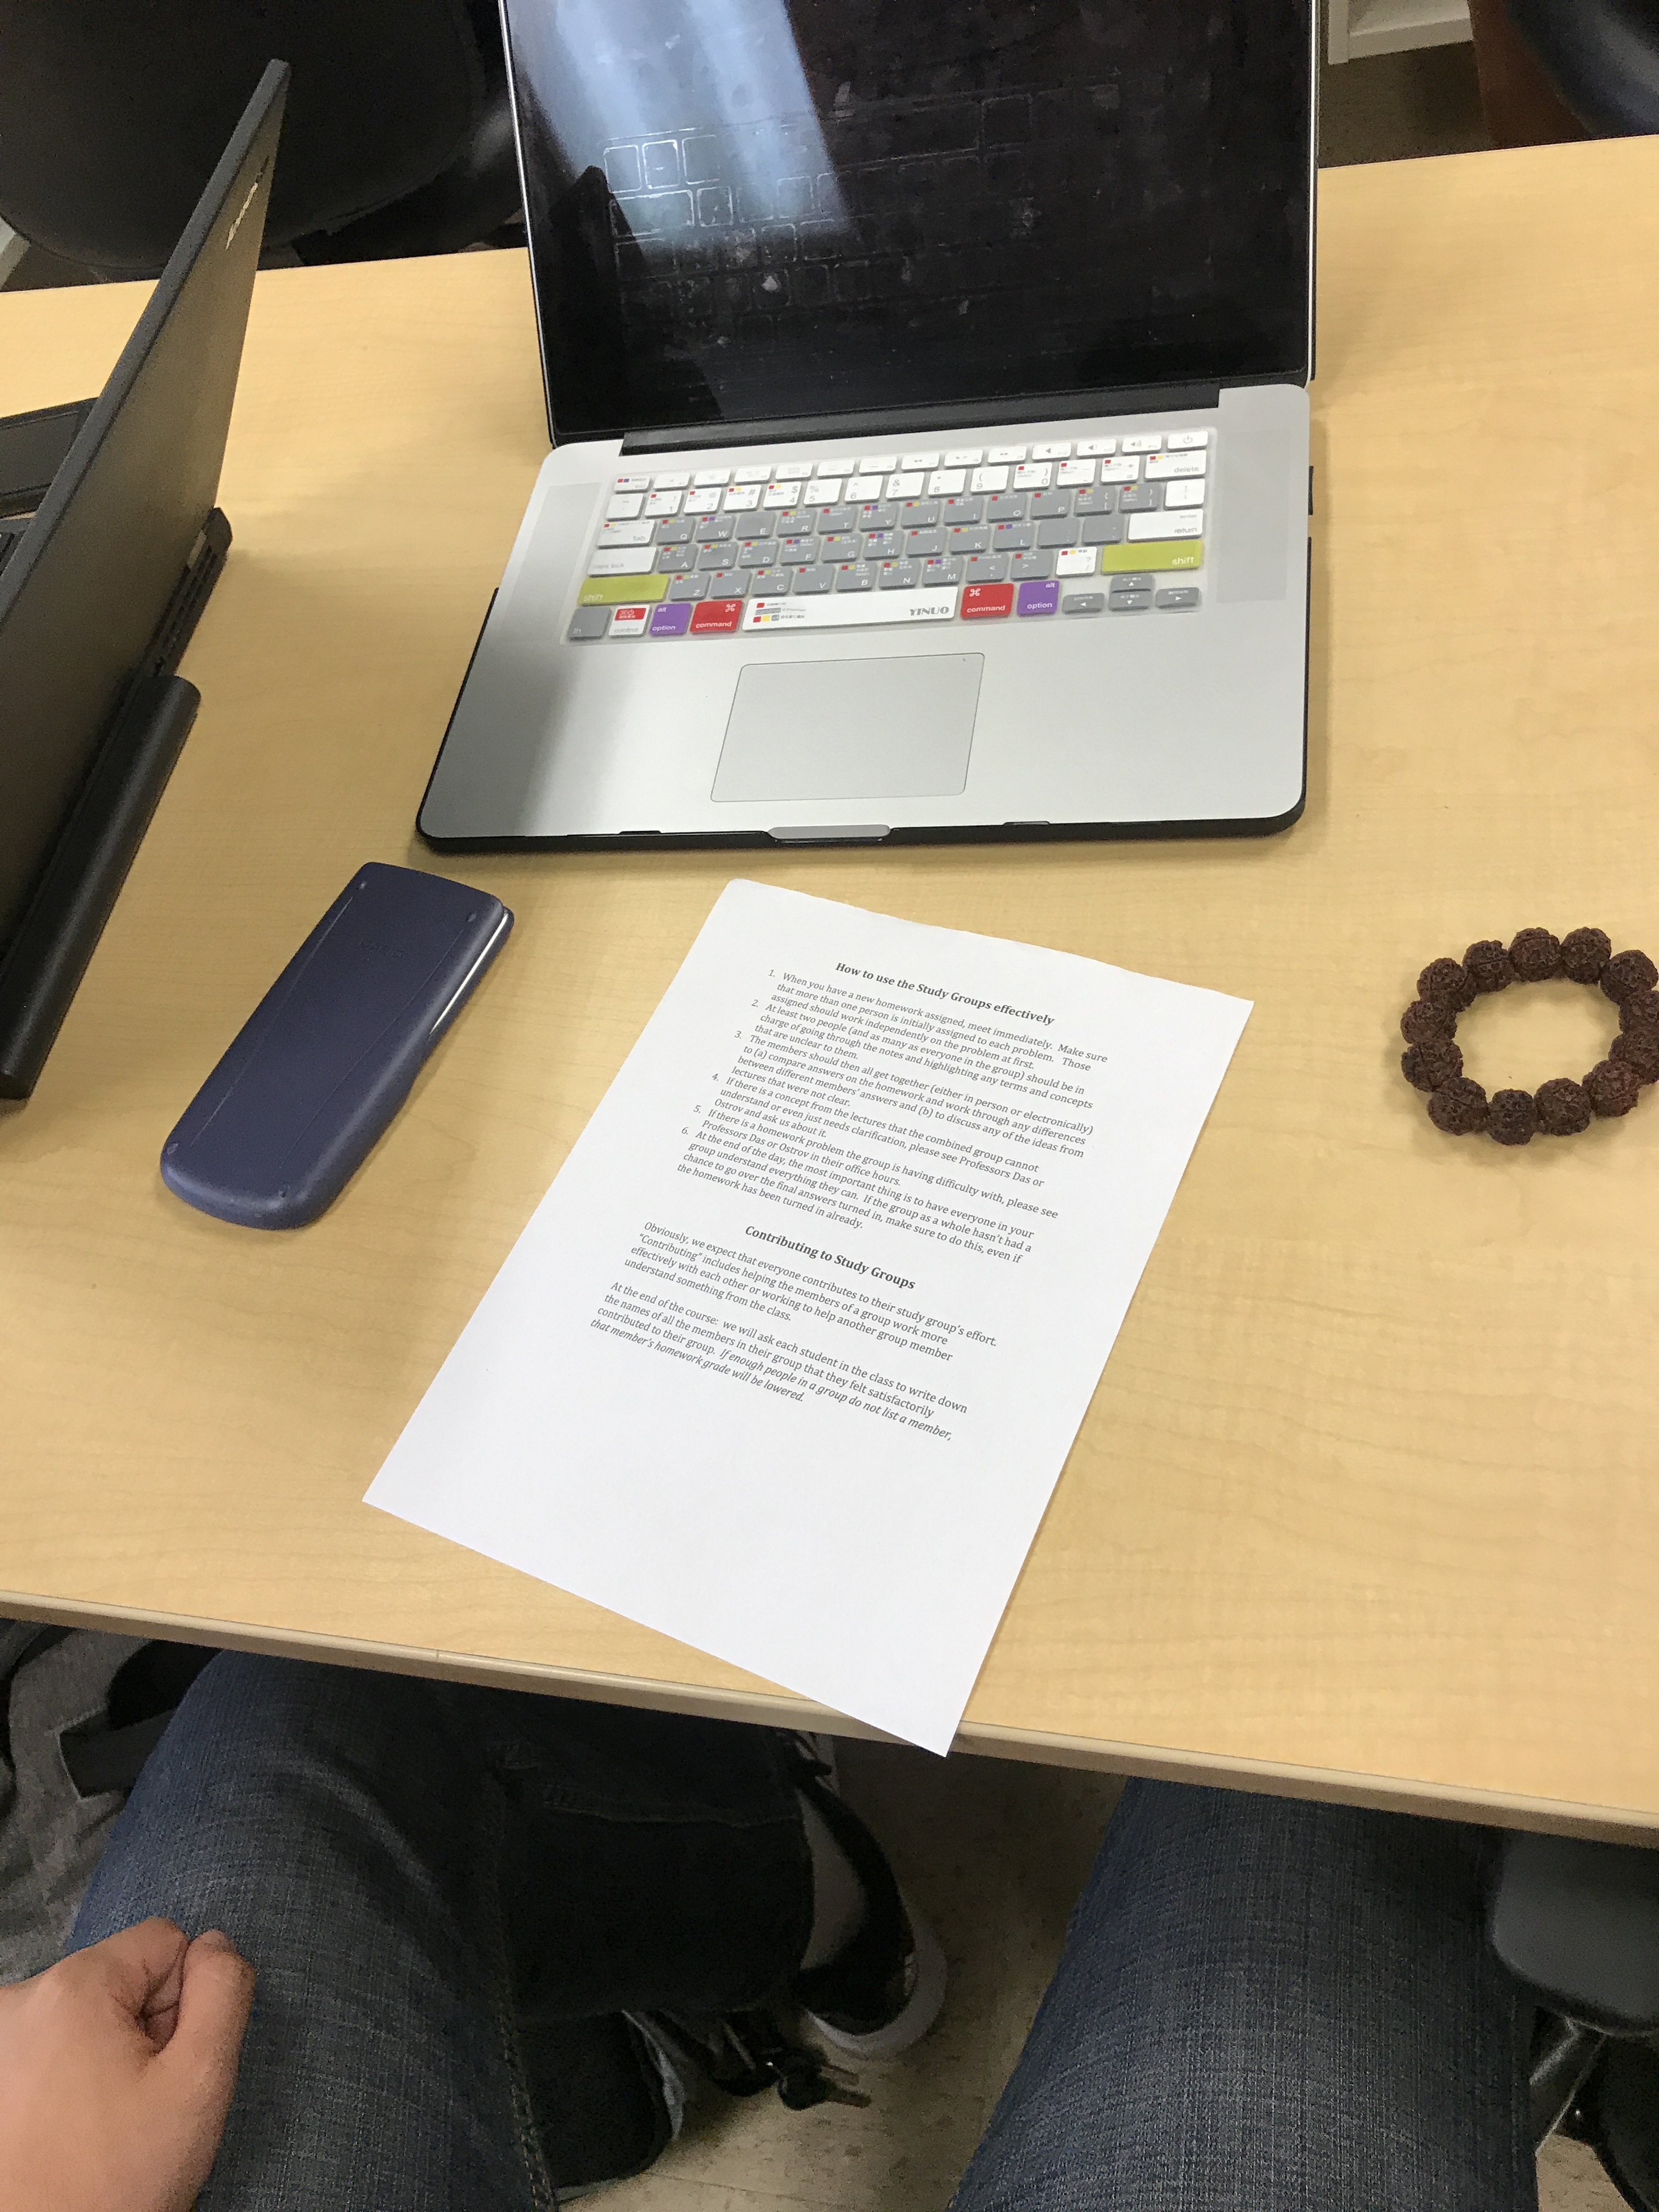
\includegraphics[width=.4\linewidth]{similar1.JPG}\hfill
	  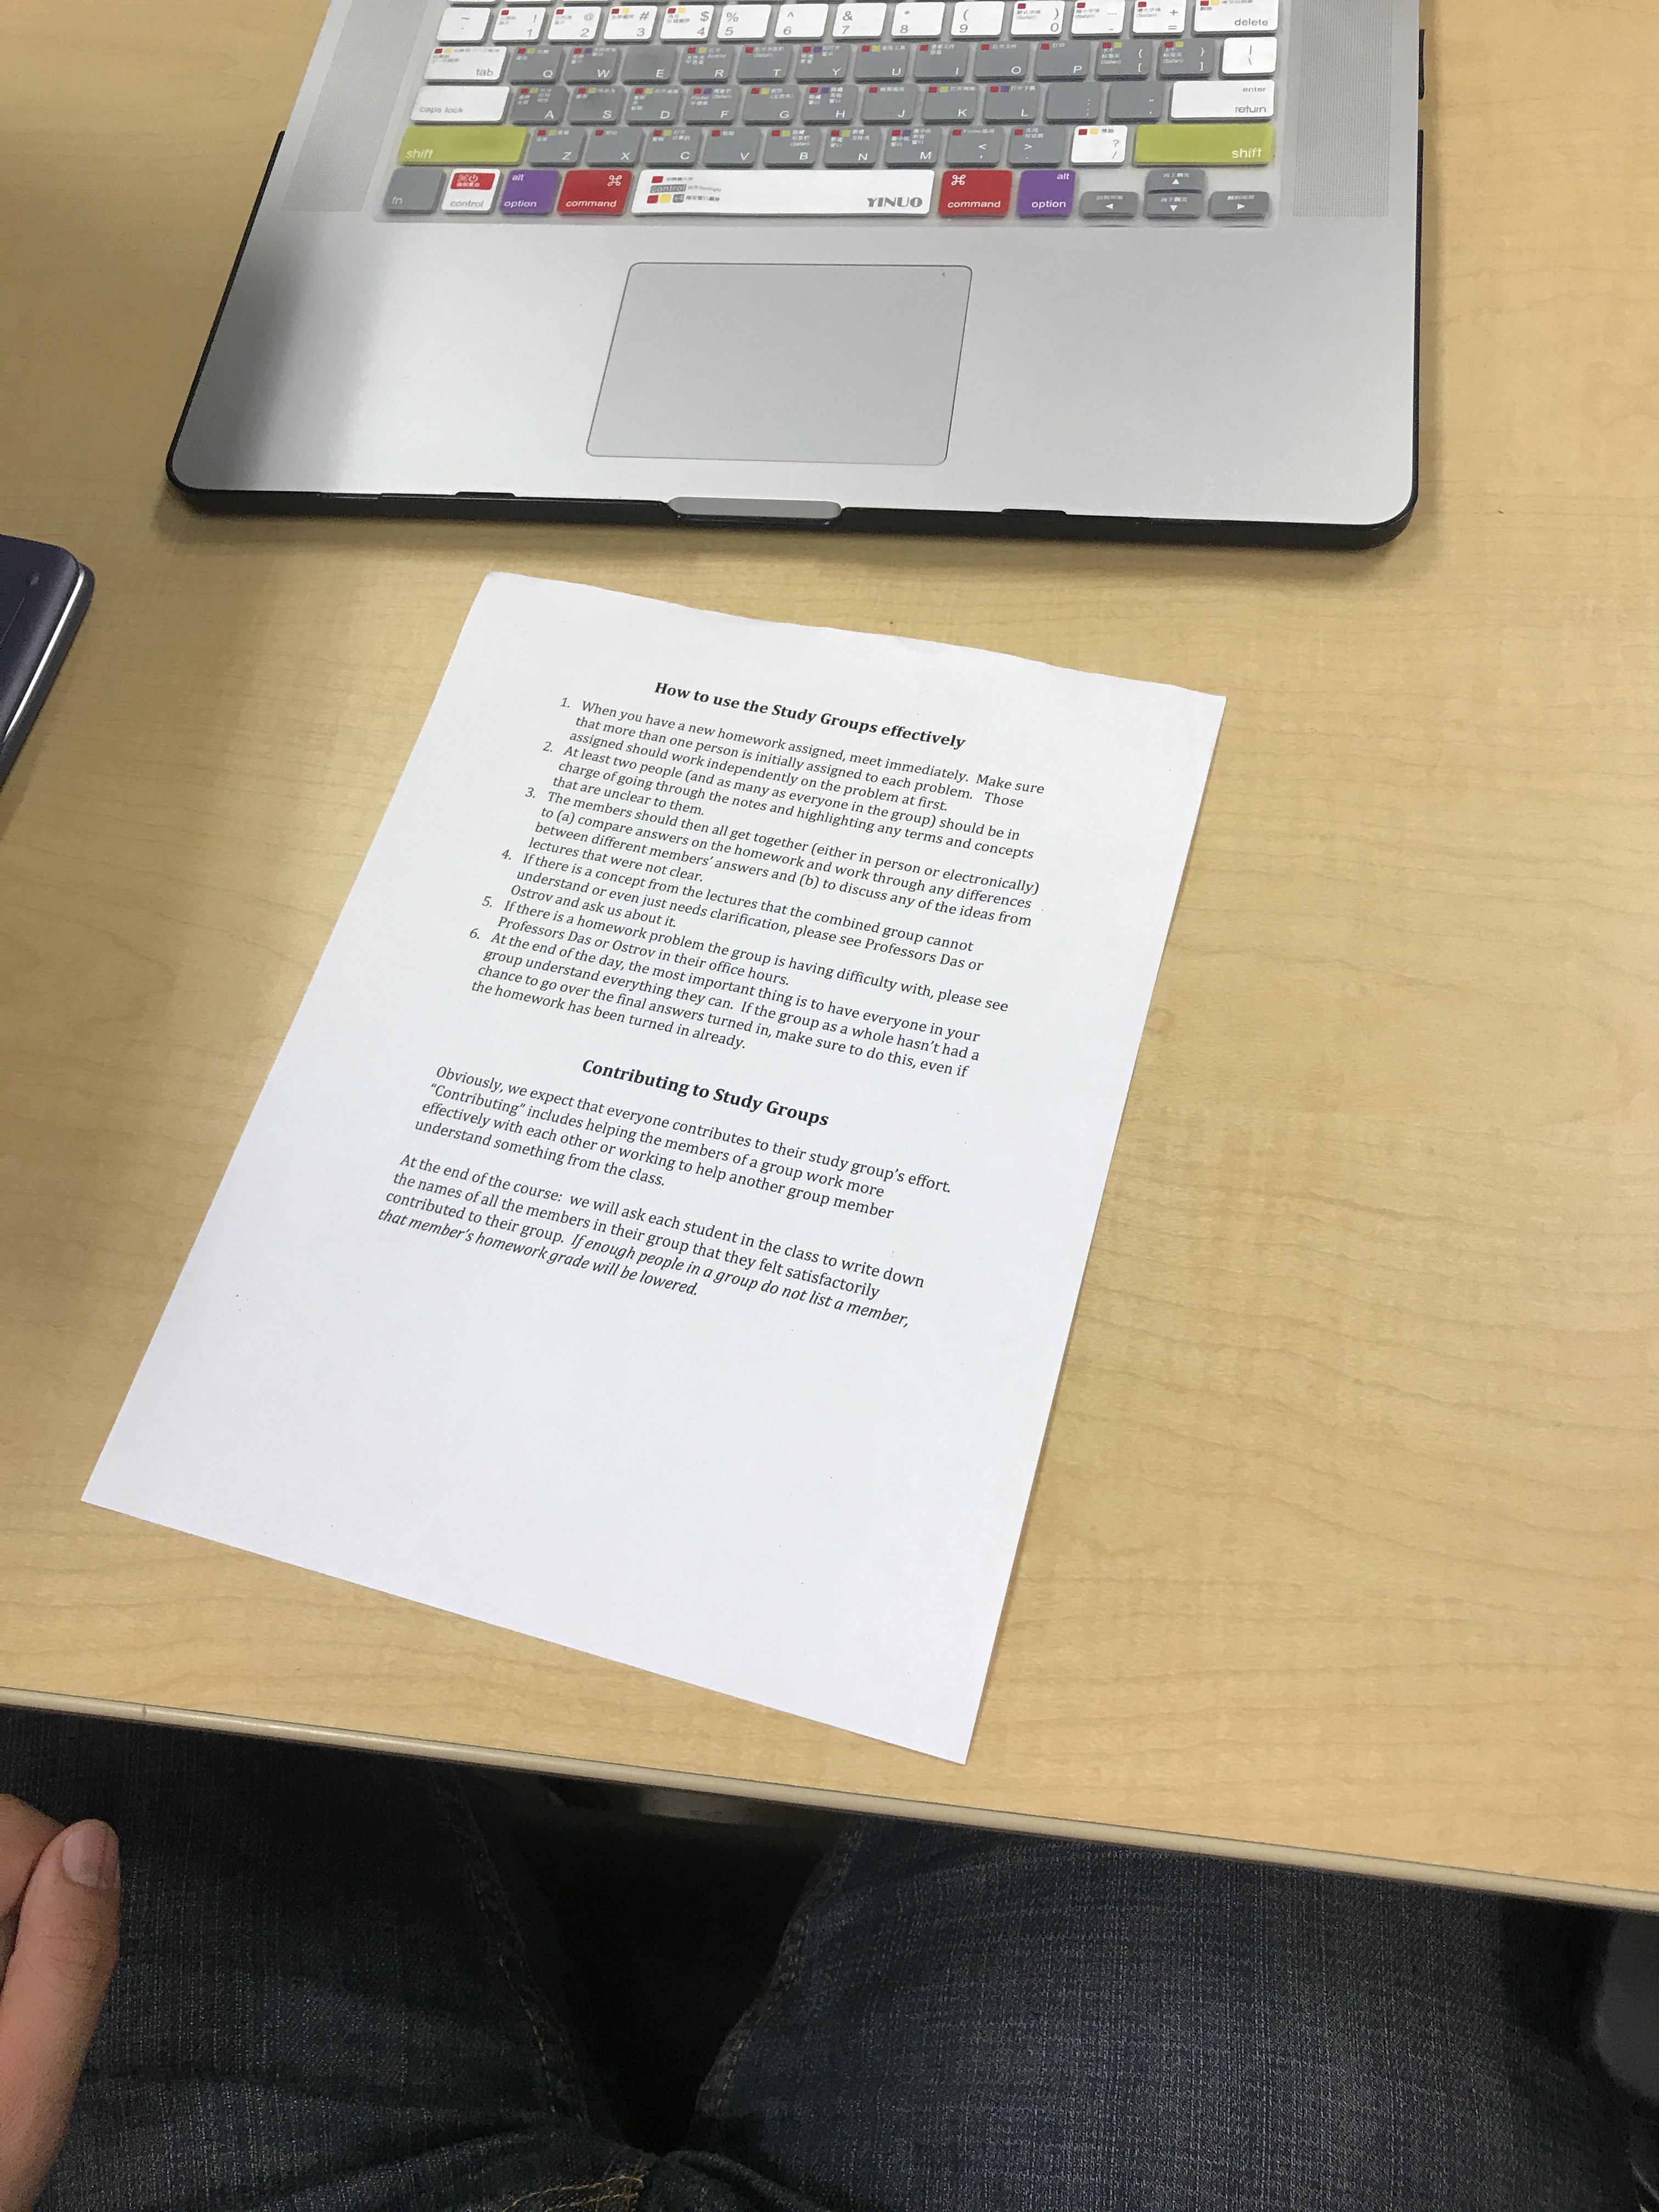
\includegraphics[width=.4\linewidth]{similar2.JPG}
  \end{subfigure}\par\medskip  
  
    \caption{Similar Images}
	\label{similarImages}
\end{figure}

\subsection{Image Processing}
\begin{figure}
	\centering
    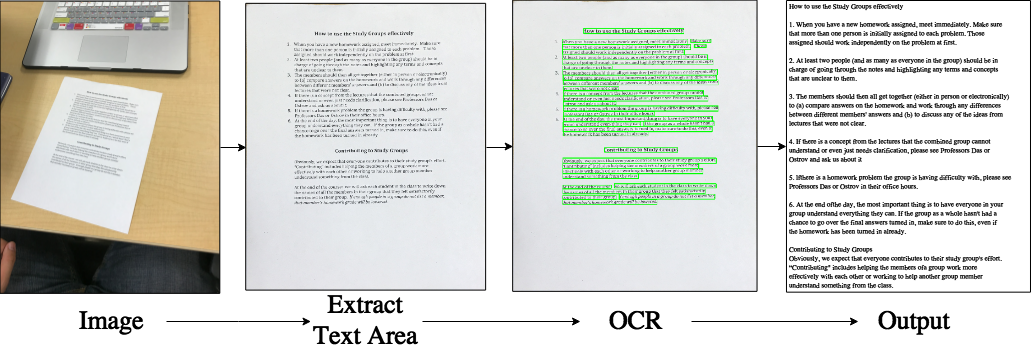
\includegraphics[scale = 0.4]{ImageProcess.png}
    
    \caption{Image Process Flow}
	\label{imageProcessFlow}
\end{figure}
When the image passed the blurriness test and the similarity test, the system will try to detect the text area in the image and extract the text area. The extracted text area is then sent to the Tesseract Optical Character Recognition (OCR) Engine to convert the image to computer encoded characters. (see Figure~\ref{imageProcessFlow})

\subsubsection{Text Area Extraction}
\begin{figure}
	\centering
    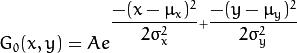
\includegraphics[scale = 1]{gaussianBlur.png}
    
    \caption{Gaussian Blur Equation}
	\label{GaussianBlurEquation}
\end{figure}
To extract the text area, a copy of the image is first blurred (5x5 Gaussian Blur is used in implementation \cite{gaussianBlur}) to detect the edges in the image (Canny Edge Detection is used in implementation \cite{canny}). From the edges of the image, contours are then collected \cite{contours} from the connected edges and sorted in descending order based on their area.

From the list of sorted contours, the biggest contour that can be approximated to a quadrilateral is identified as the text area. The text area is then applied with a perspective transformation to convert the text area to a rectangle	 as if the document is scanned. This increases the accuracy of the result from Tesseract OCR Engine. 

\subsubsection{Text Detection}
The transformed text area is processed by the Tesseract OCR Engine to identify the bounding boxes of the text in the image and convert the image to computer encoded characters. The computer-encoded characters are then processed to extract key features and feedback to the user.

\section{Text Summarization}
In order to provide users with a summary of the extracted text we use an algorithm called Term Frequency-Inverse Document Frequency \cite{tfidf} ~(TFIDF). The reason why TFIDF was chosen for our text summary is because it's one of the more popular and well known term-weighting schemes, it's easy to implement, and once it's set up it is computationally fast.

The goals of TFIDF are to obtain statistically important keywords from a text article. 

It does this by giving each word in the target document a score based on two statistics, the word frequency and the inverse document frequency.

The word frequency is simply the number of times the word appears in the target document and the inverse document frequency is calculated by taking the log of the total number of documents in a text corpus (described below) divided by the number of documents that the word appears in.

The final score for each word is calculated as follows: 

	\forceindent $tf(t, d) * idf(t, D)$  

where,

	\forceindent $tf(t, d) = 1$ if term $t$	is in Document $d$ else it's $0$

	\forceindent $idf(t, D) = log(\frac{N}{|d \in D : t \in d|}$

where,

	\forceindent $N$ is the number of documents in the corpus $N = |D|$

	\forceindent ${|d \in D : t \in d|}$: number of documents where the term $t$ appears.

The rationale behind the TFIDF algorithm is to reduce the importance of words that appear often yet have no overall significance. Examples of such words are: the, and, is, etc.


The corpus of documents are gathered in the news domain so that our text summarization is inline with the domain of PRAHVI functional requirements. Our strategy was to build our corpus by scraping the top online news repositories for all of there news articles. 

We took the 50 top online news websites. We used a Python library called Newspaper to gather the content of every article currently exists on the site.

Once our corpus was collected we precomputed the inverse document frequencies for each term in our corpus.

\chapter{Design Rationale}

	\section{Architecture}
		\begin{itemize}
			\item Hardware
			\begin{itemize}
				\item Wired video module to the phone
				\begin{itemize}
					\item Low-Latency, and therefore improving the system’s responsiveness when providing feedback to user
				\end{itemize}
				\item Choice of Haptics + Sonics Feedback
				\begin{itemize}
					\item Haptics allow us to better communicate spatial information regarding their gaze and important text or a user’s text of interest
					\item Sonics are natural way of communicating textual information to a user
				\end{itemize}
			\end{itemize}


			\item Software
			\begin{itemize}
				\item Image processing before Optical Character Recognition
				\begin{itemize}
					\item Current Tesseract OCR Engine does poorly with text that is skewed, and therefore the image processing will allow us to deskew the image as best as possible to improve performance of the OCR engine.
				\end{itemize}
			\end{itemize}
		\end{itemize}
\pagebreak
	\section{Technologies}
		\begin{itemize}
			\item Tesseract Optical Character Recognition Engine
			\begin{itemize}
				\item Currently, the most accurate open source solution to optical character recognition.
				\item Highly documented with academic papers written about it’s architecture
				\item Constantly being developed by a community of developers, so if we run into problems we have a community to ask questions to
				\item Has both a C (python wrapper) and a C++ API
				\item Supported by Google
			\end{itemize}

			\item OpenCV
			\begin{itemize}
				\item De Facto standard software libraries for computer vision
				\item Lots of developer support
				\item Open source
				\item All of its data structures are compatible with Tesseracts API
			\end{itemize}

%			\item TensorFlow
%			\begin{itemize}
%				\item Supported by Google
%				\item Scalable to distributed systems
%				\item Machine Learning Lead has most experience with this technology
%				\item Many examples of state of the art models implemented in TensorFlow making it easy to build upon, expand and even customize models to an application’s requirements
%			\end{itemize}
%
%			\item Numpy
%			\begin{itemize}
%				\item Computationally efficient way of storing and computing operations involving vectors and matrices. Useful in our application because video frames and words are commonly represented and manipulated via vectors and matrix operations
%			\end{itemize}
%\pagebreak
%			\item scikit-learn
%			\begin{itemize}
%				\item Offers state of the art plug and play machine learning models that we can use for our initial designs and provide a baseline for the performance of our system 
%			\end{itemize}
		\end{itemize}
\chapter{Testing}

	The following describes how the product is tested.

	\section{Alpha Testing}
		\subsection{Function Testing}

		During function testing, each part of the system was tested individually.
		The following are some examples of function testing performed:
		\begin{itemize}
			\item Graphical input from camera
			\item Corresponding OCR input and output
			\item Summary feedback to user
		\end{itemize}

		\subsection{System Testing}

		The system was tested as a whole. The test is focused on where all modules and functions within the system are cooperating with each other, and whether the system functions as a whole.
		
		\subsubsection{Performance}
		The performance of the system is tested with a test set of 30 images (see Figure~\ref{testImages}) with both versions of Tesseract OCR – Tesseract 3.05.00\footnote{https://github.com/tesseract-ocr/tesseract/wiki} and Tesseract 4.00.00.\footnote{https://github.com/tesseract-ocr/tesseract/wiki/4.0-with-LSTM}
		
		The test results (see Table~\ref{performanceAnalysis}) show that Tesseract 4 provides significant better results than Tesseract 3, even though Tesseract 4 is still in alpha stage.
		
		The documents in the test images are collected from BBC News (www.bbc.com). This way the ground truth of the document (the original computer encoded characters) can be used to compare with the result of the system.
		
The test images cover a variety of different backgrounds, motions, blurriness and brightness. 
		
\begin{figure}
  \begin{subfigure}{\linewidth}
  	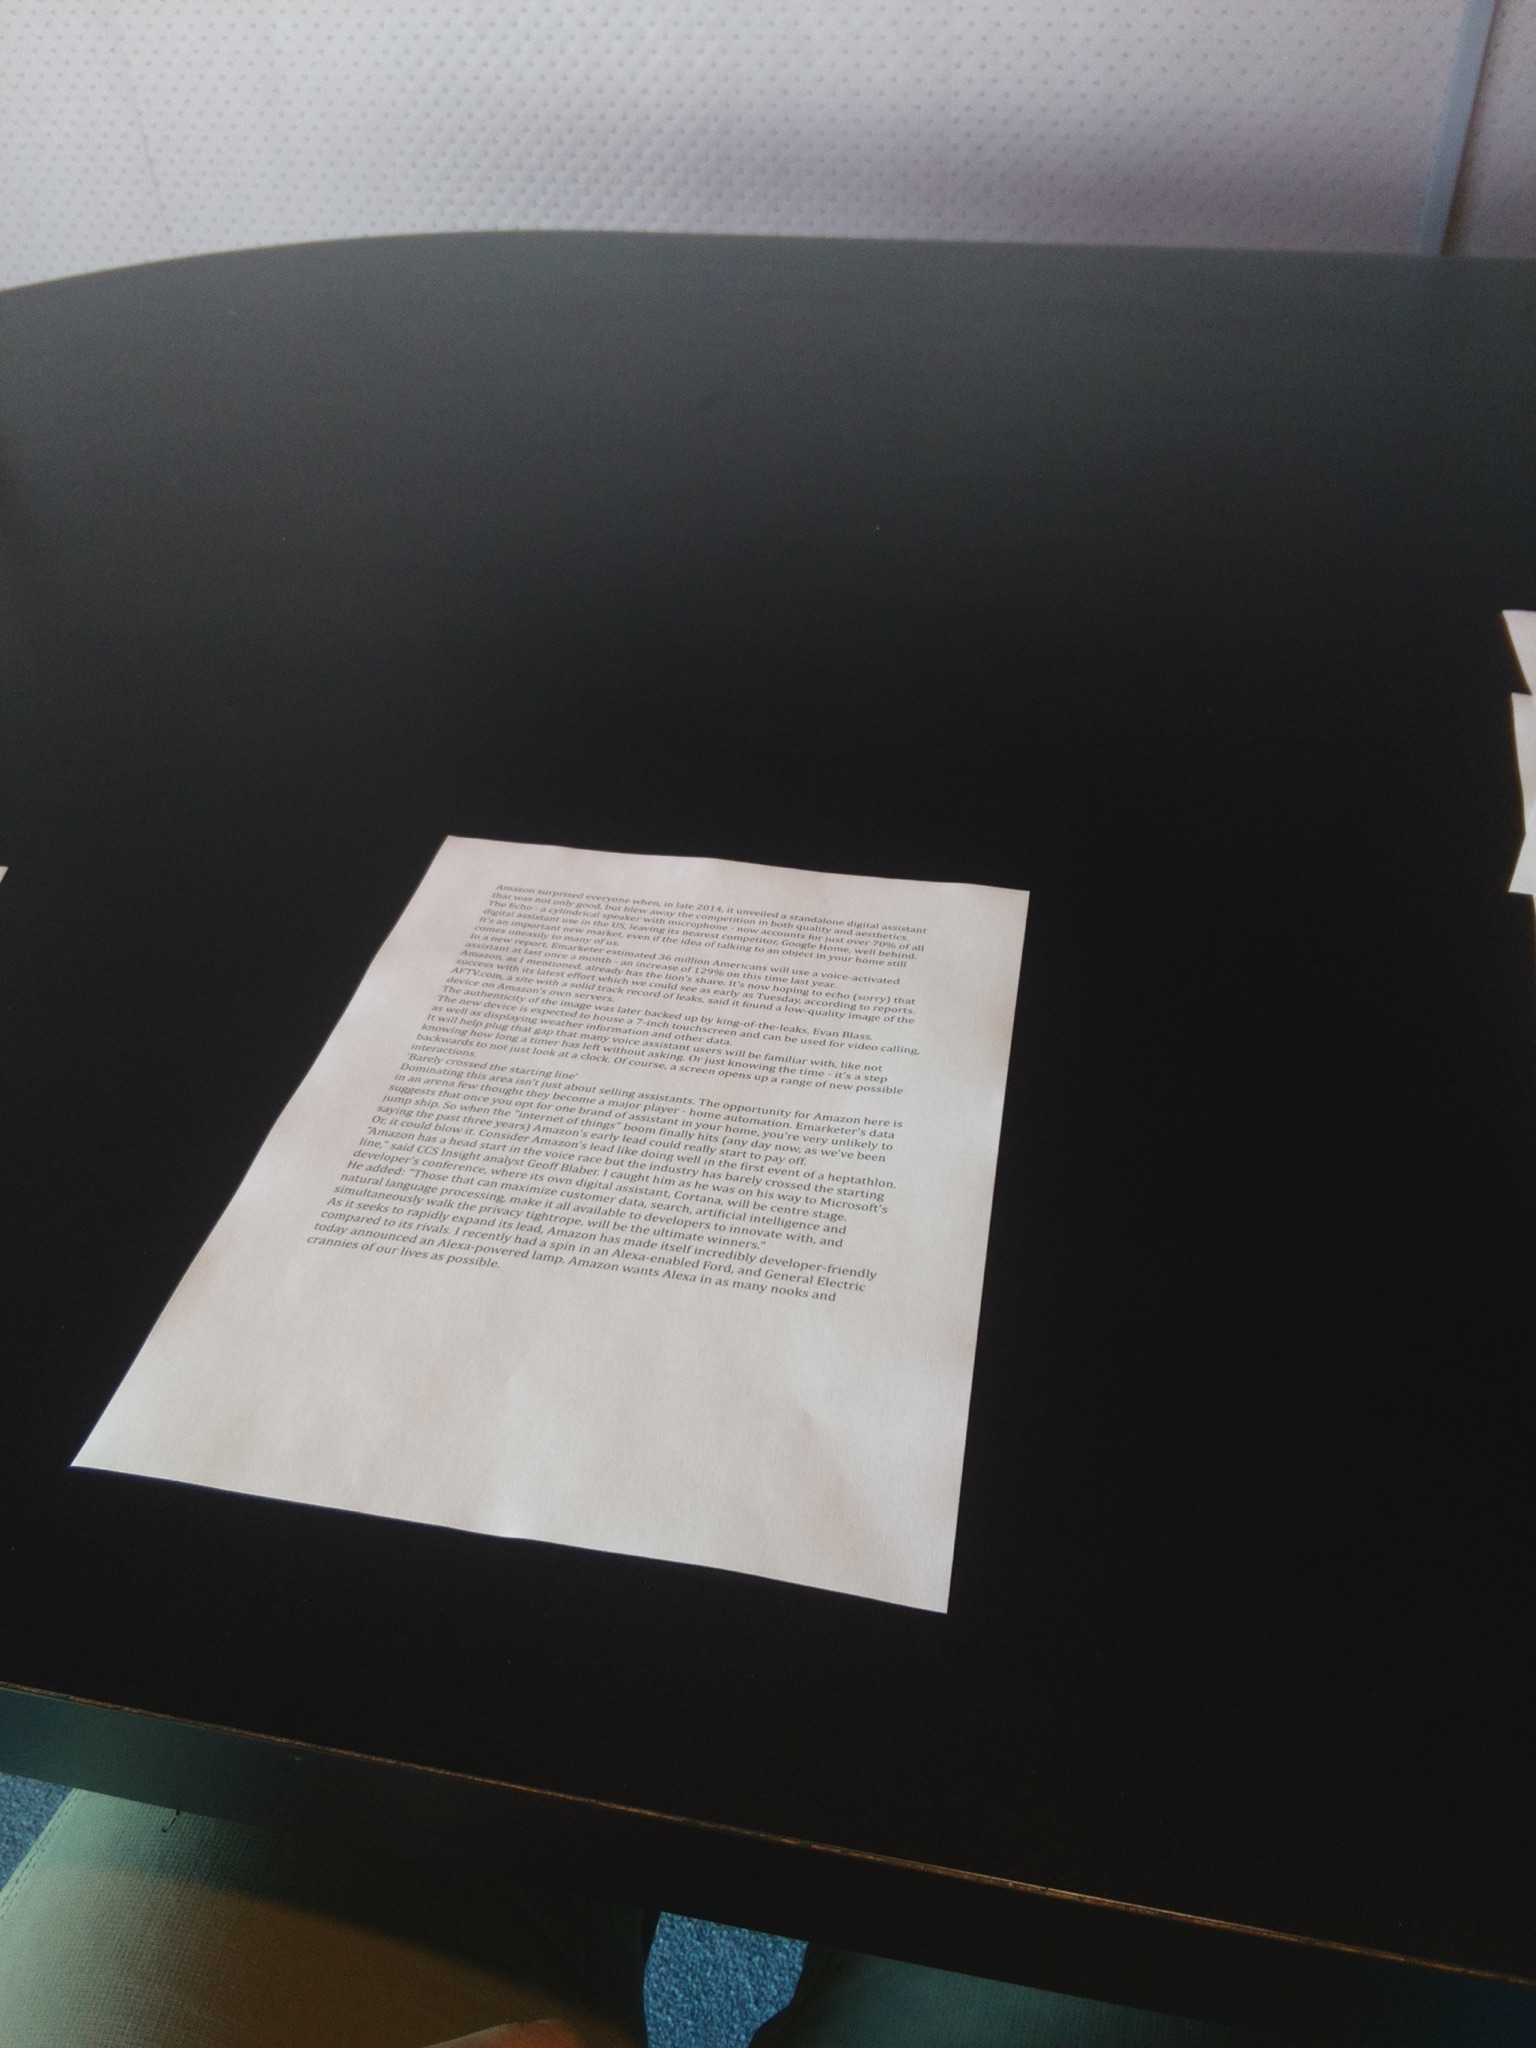
\includegraphics[width=.24\linewidth]{Amazon.jpeg}\hfill
	  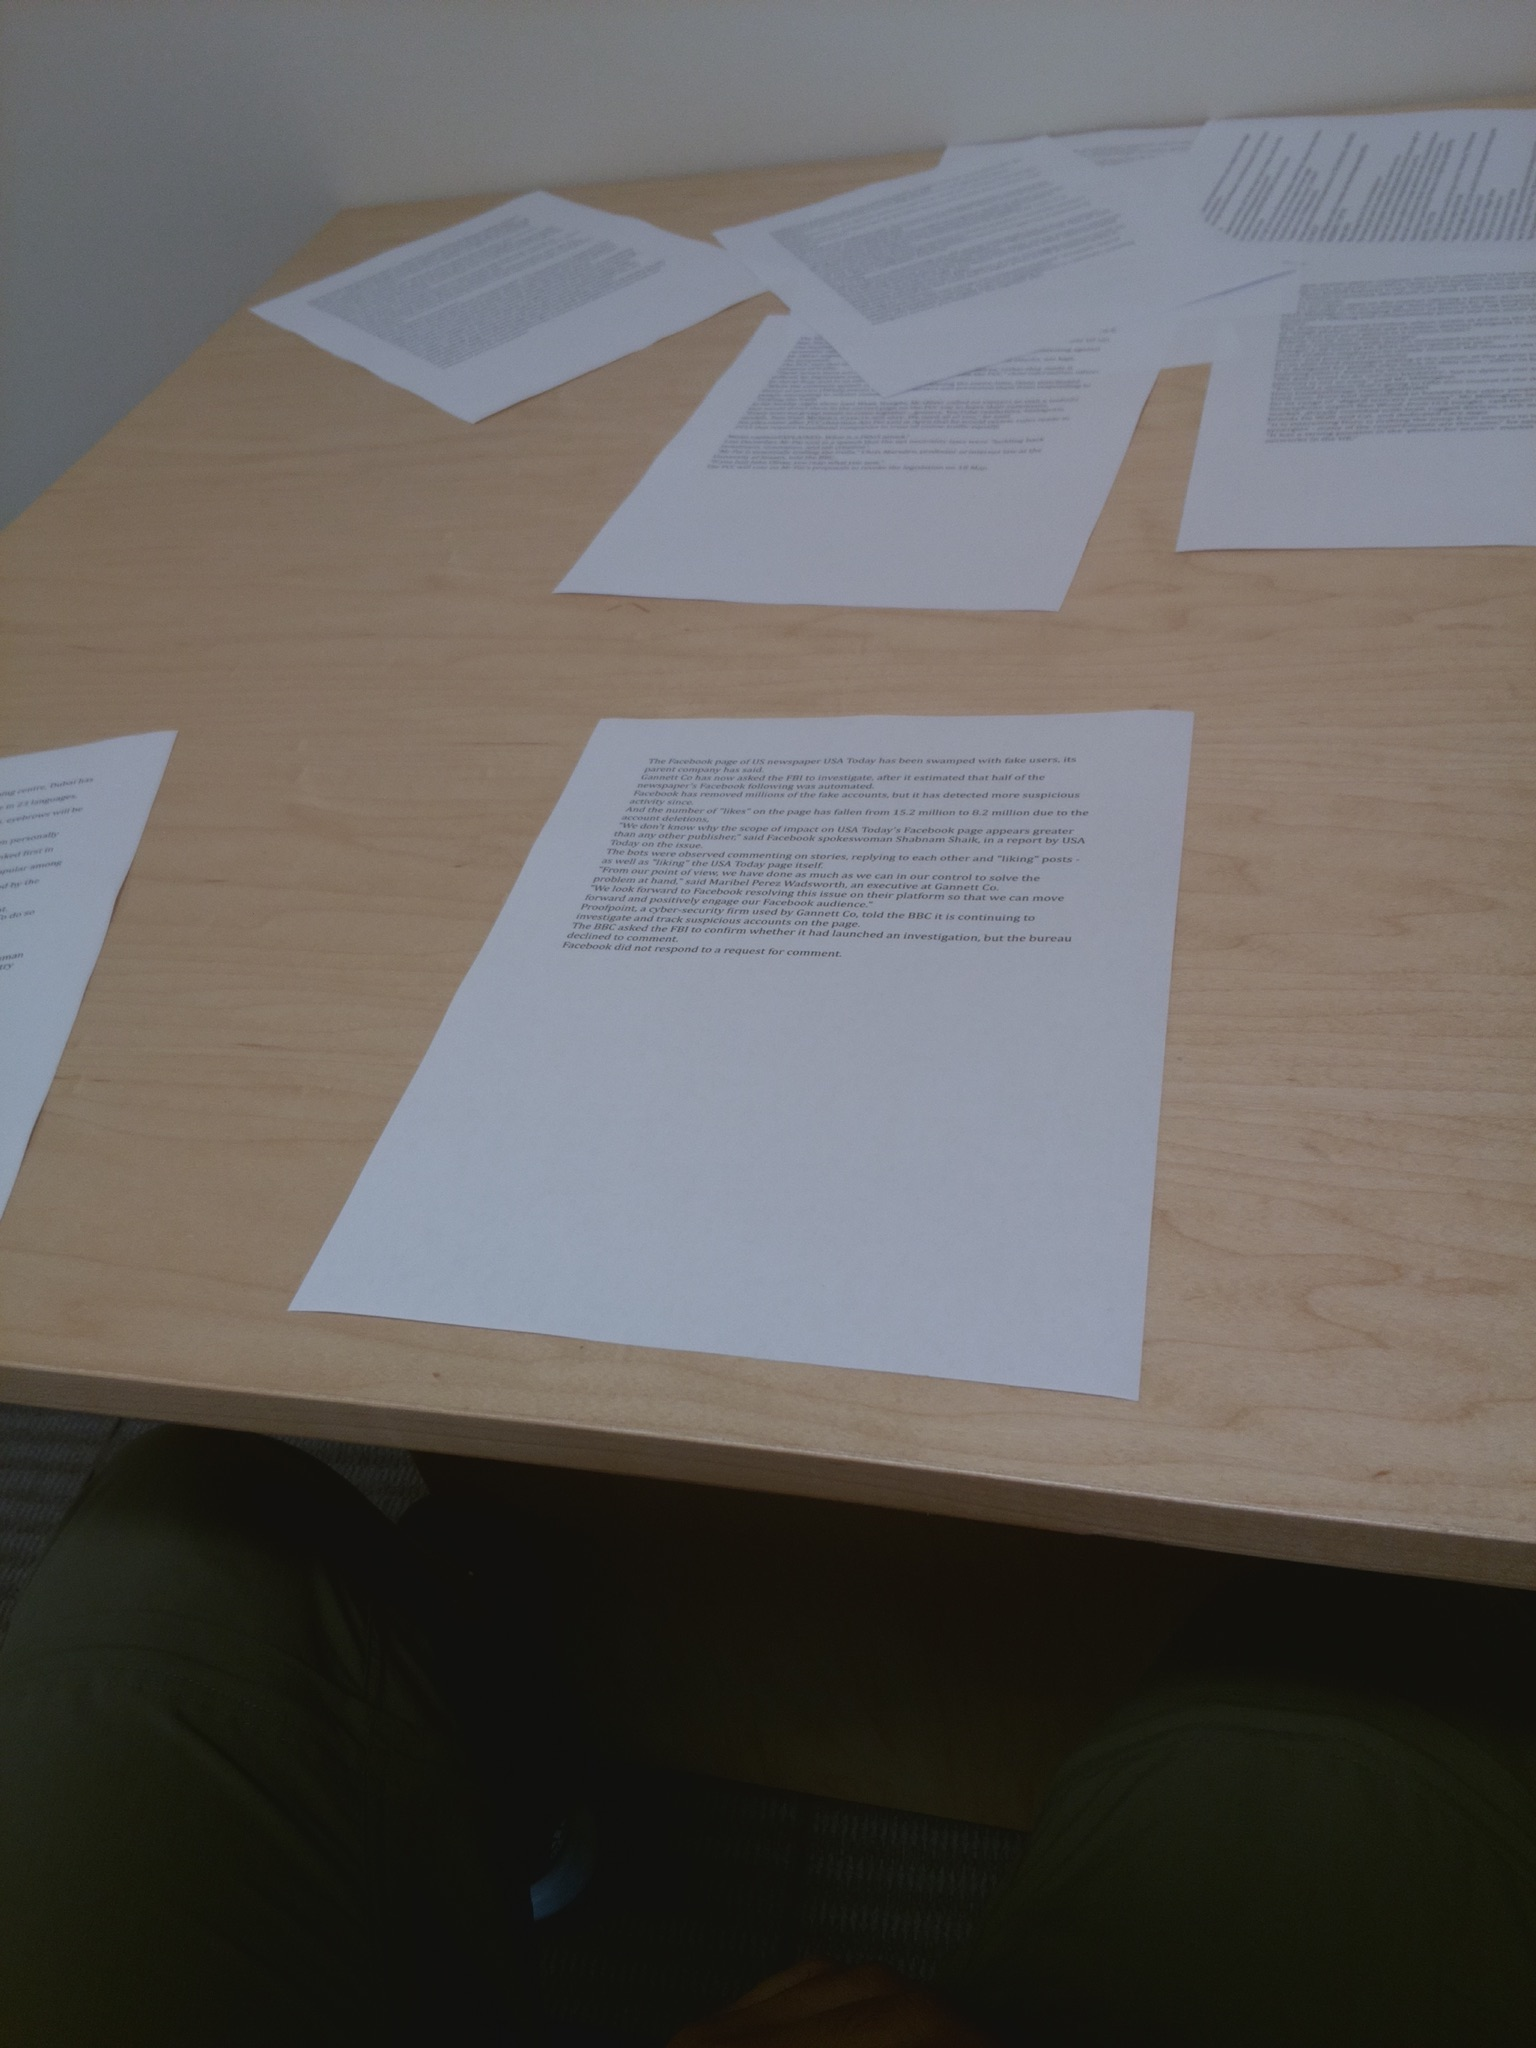
\includegraphics[width=.24\linewidth]{FacebookBot.jpeg}\hfill
	  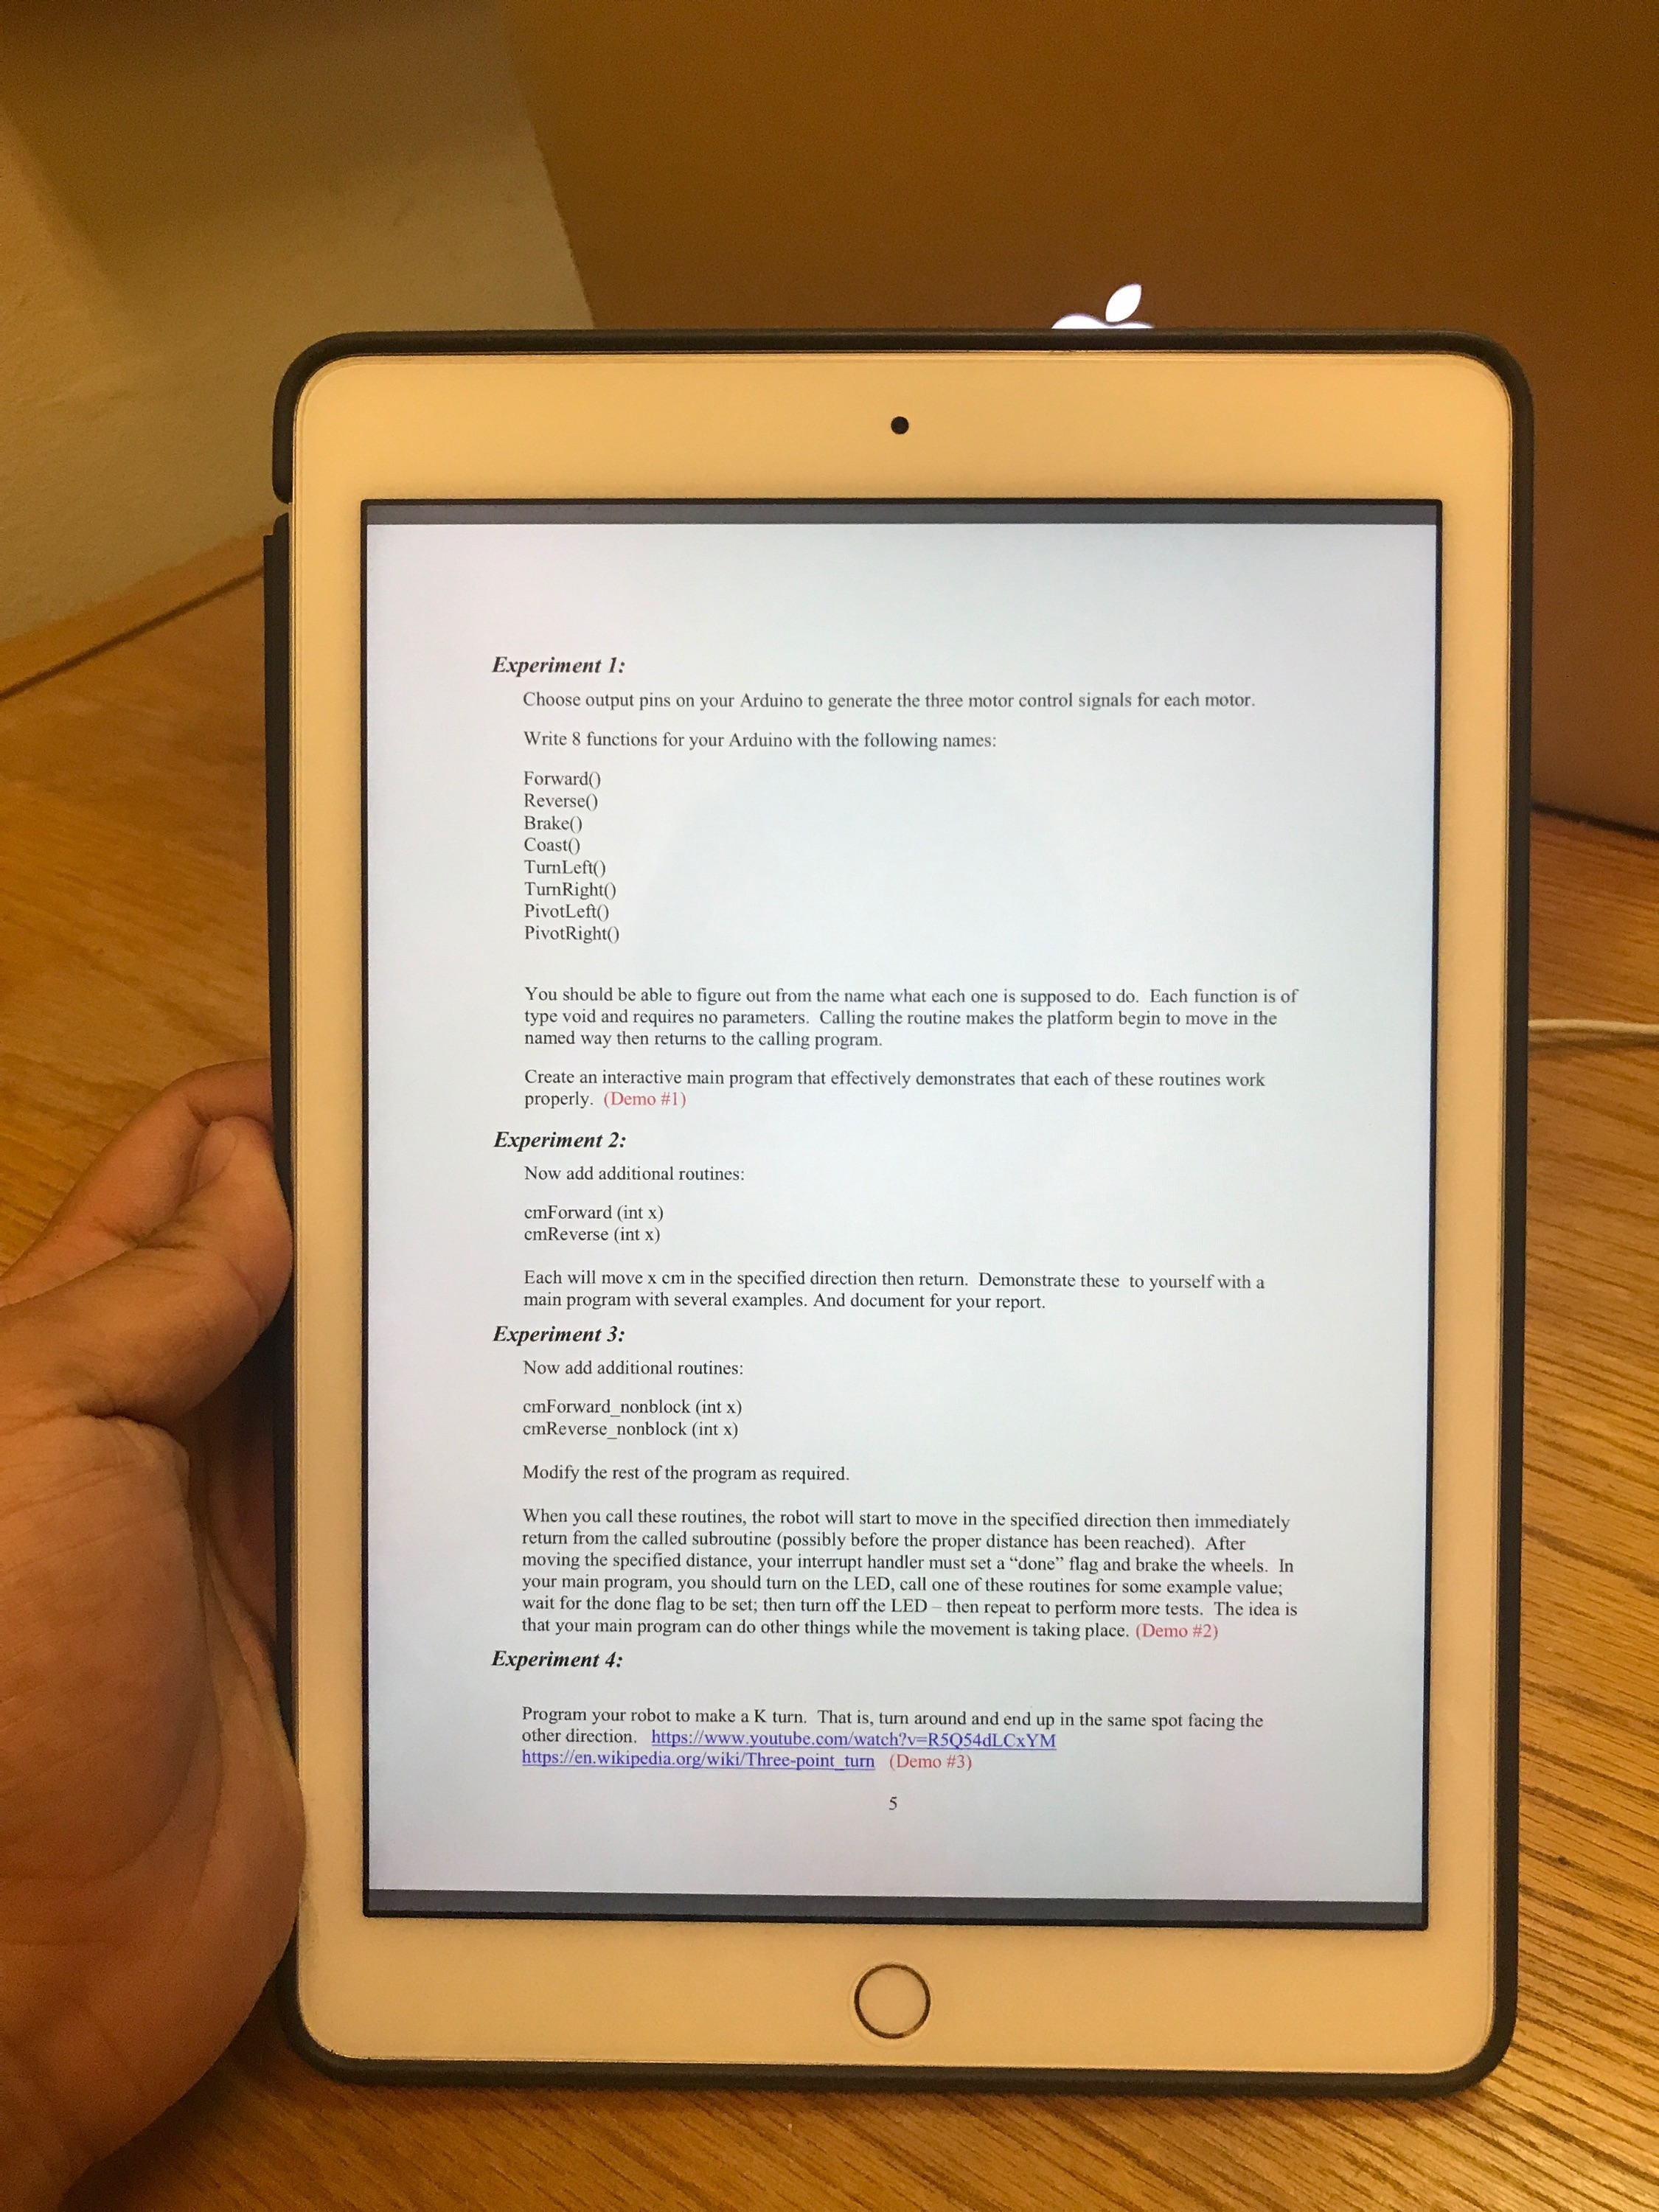
\includegraphics[width=.24\linewidth]{IMG_9203.jpeg}\hfill
	  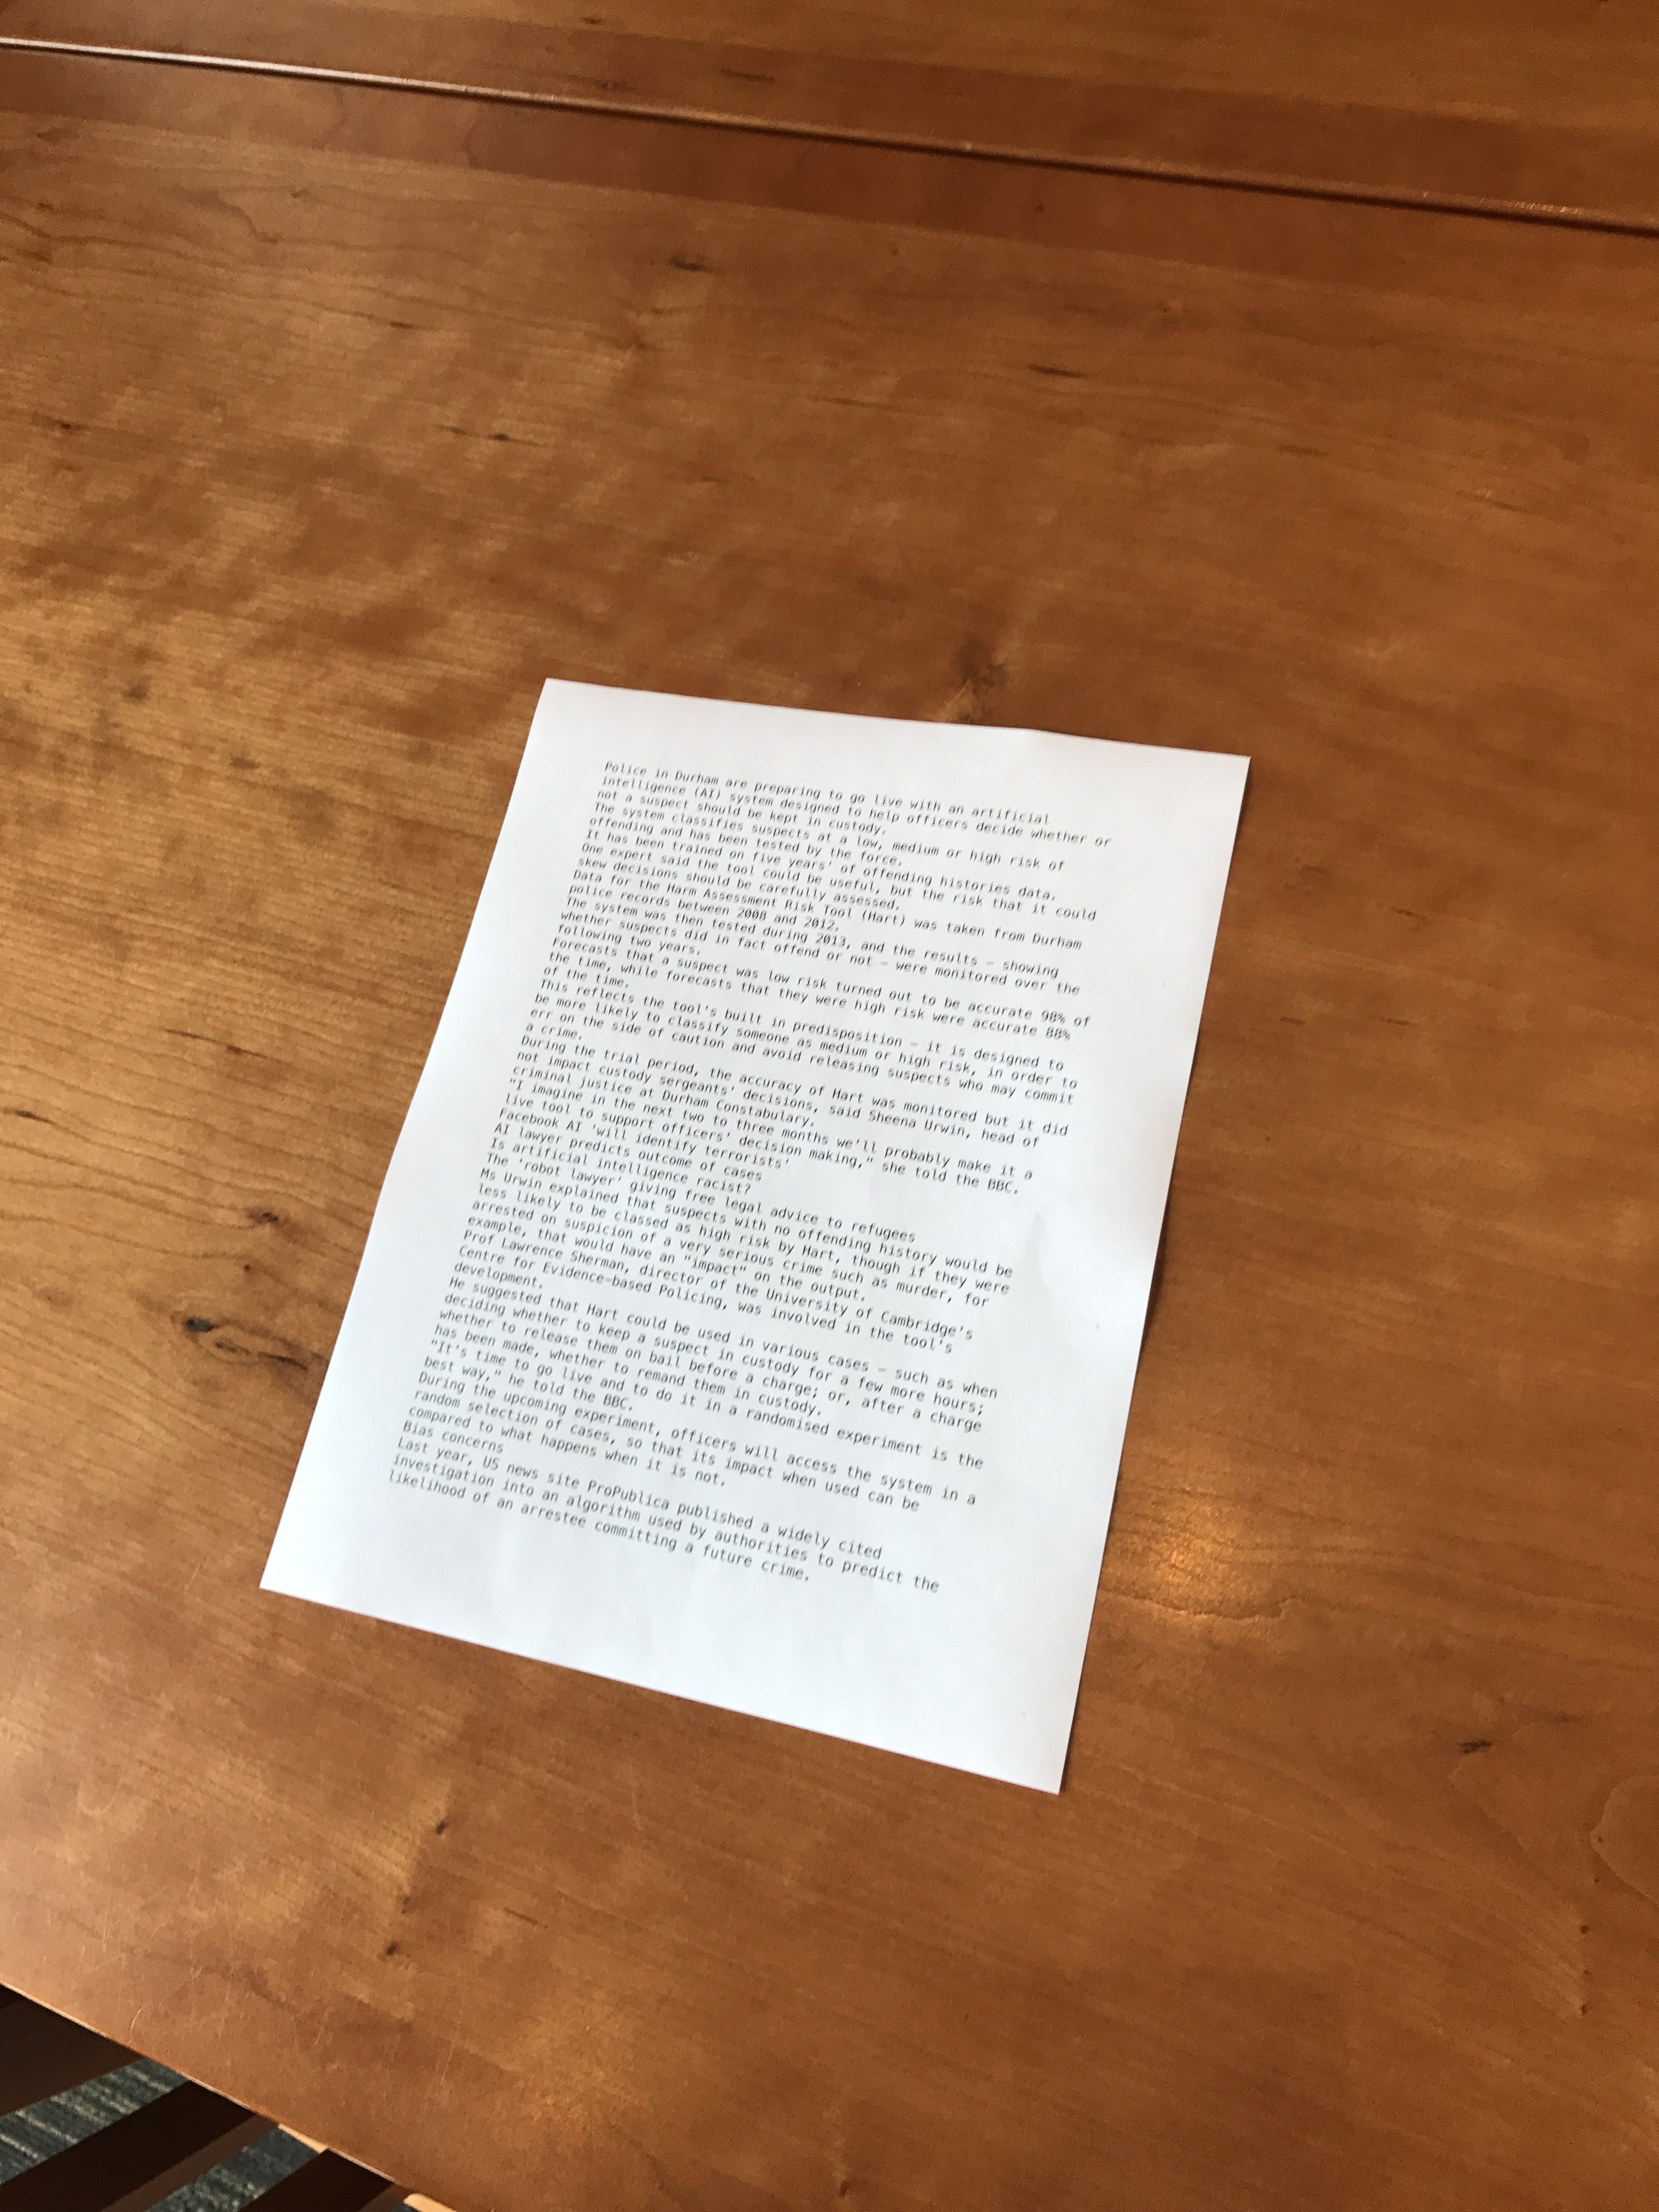
\includegraphics[width=.24\linewidth]{IMG_9259.JPG}
  \end{subfigure}\par\medskip  
  
  \caption{Testing images gathered during System Testing}
  \label{testImages}
\end{figure}


		
\begin{table}[]
\centering
\caption{Performance Analysis}
\label{performanceAnalysis}
\begin{tabular}{l|l|l|l|l|}
\cline{2-5}
\multirow{2}{*}{}                          & \multicolumn{2}{c|}{\textbf{Accuracy (\%)}} & \multicolumn{2}{c|}{\textbf{Response Time (Sec)}} \\ \cline{2-5} 
                                           & Mean           & Standard Deviation         & Mean              & Standard Deviation            \\ \hline
\multicolumn{1}{|l|}{\textbf{Tesseract 3}} & 35.93          & 21.37                      & 11.05             & 4.68                          \\ \hline
\multicolumn{1}{|l|}{\textbf{Tesseract 4}} & 91.07          & 7.24                       & 3.07              & 0.60                          \\ \hline
\end{tabular}
\end{table}

	\section{Beta Testing}
	The product was tested by visually impaired students on campus of Santa Clara University for actual user feedbacks.
\chapter{Risk Analysis}
	The Risk Analysis table defines a potential set of risks that our group could face, resulting in setbacks to timely progression towards our finished project. For each risk, there are two potential consequences, a probability value (0$\rightarrow$1), a severity value (0$\rightarrow$10), an impact value (impact=probability*severity), and two potential mitigation strategies. The risks are ordered from greatest to least impact value (top-to-bottom).

\begin{table}[]
\centering
\caption{Risk Table}
\label{riskTable}
\begin{tabular}{|l|l|r|r|r|l|}
\hline
\multicolumn{1}{|c|}{\textbf{Risk}}                                                                       & \multicolumn{1}{c|}{\textbf{Consequences}}                                                           & \multicolumn{1}{c|}{\textbf{Probability}} & \multicolumn{1}{c|}{\textbf{Severity}} & \multicolumn{1}{c|}{\textbf{Impact}} & \multicolumn{1}{c|}{\textbf{Mitigation Strategies}}                                                                                                                                                                     \\ \hline
\begin{tabular}[c]{@{}l@{}}Software platforms or\\ hardware are difficult\\ to link together\end{tabular} & \begin{tabular}[c]{@{}l@{}}Development\\ blocked\end{tabular}                                        & 0.5                                       & 9                                      & 4.5                                  & \begin{tabular}[c]{@{}l@{}}Use common, open-source\\ platforms that have supports.\\ Modulize the system, such \\ that every part can be\\ replaced easily.\\ Communicate effectively\\ with team members.\end{tabular} \\ \hline
Low content accuracy                                                                                      & \begin{tabular}[c]{@{}l@{}}System becomes\\ less accurate\end{tabular}                               & 0.4                                       & 8                                      & 3.2                                  & \begin{tabular}[c]{@{}l@{}}Make good use of user\\ interaction such that the\\ device may instruct the user\\ to reposition to getter better\\ results and rely on the\\ expertise of advisors\end{tabular}             \\ \hline
\begin{tabular}[c]{@{}l@{}}Long response\\ turnaround time\end{tabular}                                   & \begin{tabular}[c]{@{}l@{}}Long wait time\\ for the user\end{tabular}                                & 0.4                                       & 7                                      & 2.8                                  & \begin{tabular}[c]{@{}l@{}}Implement the system such\\ that it is able to transfer to\\ faster framework or more\\ powerful hardware\end{tabular}                                                                       \\ \hline
\begin{tabular}[c]{@{}l@{}}Too hard to get good\\ environment with light\end{tabular}                     & \begin{tabular}[c]{@{}l@{}}Unable to get\\ performance data\\ Result is less\\ accurate\end{tabular} & 0.5                                       & 3                                      & 1.5                                  & \begin{tabular}[c]{@{}l@{}}Use camera than can\\ change the focus, exposure\\ and white balance when\\ capturing the image\end{tabular}                                                                                 \\ \hline
\begin{tabular}[c]{@{}l@{}}Too narrow a range of\\ operability\end{tabular}                               & \begin{tabular}[c]{@{}l@{}}System becomes\\ less useful\end{tabular}                                 & 0.3                                       & 4                                      & 1.2                                  & \begin{tabular}[c]{@{}l@{}}Implement the system that\\ is able to operate and\\ cover most situations\end{tabular}                                                                                                      \\ \hline
\end{tabular}
\end{table}

\chapter{Ethical Analysis}
	The primary goal of PRAHVI is to help individuals with visual disabilities more easily integrate into society. With millions of Americans living with some level of blindness, there was an opportunity to significantly affect a broad set of individuals with some very specific challenges. Working with the university's disabilities office, we discovered typical use cases involving navigating one's indoor environment, identifying and reading texts that have no digital equivalent, and independently interacting with one's outdoor environment. These simple tasks help individuals become more productive, opening broad opportunities for work and fuller lives. Improving any single one of these daily tasks vastly improves the quality of life for individuals in this segment.
	
	Through our ethical analysis we discovered that one of the most important attributes successful engineers have is the ability and willingness to observe their work in the broad scope of the people they affect. Although the requirements, design, and implementation of PRAHVI changed during the course of its development, the team was constantly guided by the factors that would deliver the best experience to our target users given the time and resources we have. Most notably, this included prioritizing features with a sense of those that could be completed in a reasonable timeframe while driving our primary objective. This mindset ensured the success of the project in the face of unexpected developments by focusing on the desires of the stakeholders involved.
	
	Although PRAHVI is classified as an assistive device, its usage comes with ethical implications of its operation that we took into account during the development process. The main ethical implications are ultimately predicated on the newfound independence users gain by using PRAHVI, at the potential expense of privacy or inaccurate translation. In terms of privacy, a simple case could arise when PRAHVI is used to translate sensitive information such as a bank statement or an address. As PRAHVI dictates the text it reads, the translation could be accidentally read to bystanders as well as the user. A more complex case could involve a malicious actor gaining unauthorized access to the device, by way of "hacking" it, and in turn record the sight and whereabouts of the device during usage. Such information could compromise the user's sensitive information or place him or her at risk of other attacks such as fraud or assault. These factors were taken into account during the development of PRAHVI and its software architecture to ensure that the risk for stakeholders is minimized.

\chapter{Sustainability}
	Sustainability is an essential factor in delivering a product that will benefit people's lives and create value. During the design of PRAHVI, we have identified multiple points of sustainability through the lifecycle of the product: from its environmental costs, to its user interaction, to its economic viability. By evaluating these facets, we can draw a concrete “triple bottom line” to evaluate the effectiveness of the product in the context of an actual business model.
	
	As a product, PRAHVI is designed primarily using off-the-shelf components that have been developed at scale both to reduce costs and to minimize its environmental footprint. Its construction consists mainly of a PCB board, a camera module, a plastic enclosure, and a cable to connect the product to the user's smartphone. The board used in the current version is the Raspberry Pi Zero, a lightweight, low-power board designed for mobile applications. This means that PRAHVI operates using less than 100mW and can be powered entirely by a smartphone's accessory port. The electrical components are manufactured in compliance with the global Restriction of the Use of certain Hazardous Substances (RoHS) regulation. Additionally, each company we have sourced components from have publicly pledged their products to be free of conflict materials and use minimal amounts of rare-earth metals. This allows us to minimize the environmental impact of both construction and disposal of the product by accounting for its individual materials and by following federal and international procedures. The enclosure is constructed using a 3D printer with ABS plastic material. Although this material is not biodegradable, using a pure ABS filament and designing the product to be modular allows a recycling entity to separate the components and recycle the ABS plastic. Overall, we anticipate a single PRAHVI unit to last the life cycle of the user's smartphone, typically 2-3 years. This accounts for future feature upgrades and the general durability of the product against normal wear and tear. By accounting for each of these factors during the design phase of our project, we can minimize PRAHVI's overall environmental footprint.
	
	In terms of social sustainability, we have chosen a very clear demographic that has been largely untapped for innovation. Making PRAHVI a promising product for this field. PRAHVI is designed to assist users with visual disabilities navigate their visually-oriented environments, from casual reading to discovering signs and posters. The use cases it presents are context-specific but very familiar to those who struggle with these tasks on a daily basis. Because we tailored the interface of the product to individuals with partial or full visual disability, making the product intuitive presents a unique challenge for us. By crafting an interface that communicates primarily through sound and haptic feedback, we believe that the product is intuitive and useful for the user. Furthermore, test the product through usage exercises and potentially real-world user tests. However, creating a product for this niche also introduces the possibility that users will develop an implicit dependence on the product. Should the user begin entering high-risk environments on his or her own, such as navigating a busy street, the stakes for failure could mean the difference between life or death. Therefore, for the first few iterations of the product, we would advise users only to use the product in a controlled environment with minimal hazards and many safeguards. Overall, we hope that PRAHVI can add significant value to a user's daily life with the objectives we have set, using the technologies and sense of interface we have developed.
	
	The final metric for a product's viability involves economic sustainability, particularly in a world saturated with electronic assistance devices. By utilizing off-the-shelf components and relying on a smartphone that users in this demographic typically already have, we have made strides in minimizing the cost of the product to well below current solutions. Our target cost of the product was less than \$200, which is a fraction of the closest competing product, OrCam, which is priced at \$2500. Much of the cost for such devices is in the software and the processing unit, as these devices are typically designed to be standalone. During the design phase of our project, we studied the demographic of individuals with visual disabilities and found that many typically own and use a smartphone on a daily basis. This means that we can safely trade off a small measure of convenience with a standalone device for the cost savings of using a processing unit users already own. Additionally, this drives down the cost and frequency of future upgrades, as the device's processing power is upgraded for free with every new smartphone a user purchases. This means less revenue is spent on developing and manufacturing new PRAHVI processing modules.
	
	Most of PRAHVI's revenue would go to the material cost of the components and development and testing of the software. Additionally, the retail cost to the end user can typically be augmented by support from their insurance providers. In the future, PRAHVI may be manufactured entirely using a custom PCB board and custom hardware that, at scale, would further drive down costs while delivering a more integrated product. From an economic standpoint, PRAHVI is an effective product in this segment, especially compared to competing products, by using a careful mix of tradeoffs that overall benefit users.
	
	We hope that PRAHVI meets or exceeds the “triple bottom line” to remain a fully-sustainable product. By identifying a key niche ripe for innovation, then sourcing parts and development in an environmentally and economically responsible way, we envision a life cycle that helps the product remain viable for many iterations. With each iteration, we also hope that the product can incorporate fixes and improvements that make it more useful for users and even expand its target audience. These goals overall would help create the framework for a transition from a simple design project into an actual product.
	
	In a world with increasingly limited natural resources and a larger focus on industrial impact on our environment, sustainability is a significant part of research and development. During the design of PRAHVI, we have identified processes, components, and the sourcing of these components to evaluate its environmental impact. As a product that spans multiple industries, we recognize that PRAHVI's lifecycle includes many stakeholders and resources, from manufacture, to daily usage, to final disposal.
	
	The construction of PRAHVI begins with its components, their sourcing, and overall assembly. The primary component of the device is its printed circuit board (PCB). For research purposes, we have used an off-the-shelf board known as the Raspberry Pi Zero. This board consists of plastic for the board itself, laser-etched copper traces, and components with varying amounts of copper, silicon, and gold. In compliance with the global Restriction of the Use of Certain Hazardous Substances (RoHS) regulation, the Raspberry Pi is manufactured without the use of conflict materials and minimal use of rare-earth elements. In addition, the camera module by Sony Inc. is manufactured under stricter regulations that replace many materials, such as those that go into the imaging sensor, with more environmentally-friendly, albeit slightly more expensive alternatives. We found that the small form factor of the Raspberry Pi not only makes the product more portable, but uses fewer materials, while still meeting our quality and performance requirements. Although other boards and modules were evaluated, most are manufactured under small-scale operations that use more resources or did not meet our requirements. The case of the product is manufactured using a 3D printer with ABS plastic material. This material is not biodegradable, and must be recycled at the end of the product's lifecycle. During the design phase of this project, we selected what we believe are the optimal components and materials for PRAHVI from a performance and environmental standpoint.
	
	As a holistic product, PRAHVI introduces challenges to managing energy consumption from manufacture, to delivery, and daily use. The parts used in PRAHVI are sourced primarily from China. With careful design and planning, we consolidated our parts orders into three stages and from a single supplier to ensure that we minimized the impact of transportation in the product. The case, which is manufactured using a MakerBot Replicator 2X, is the only part we manufacture ourselves. For research purposes, using a 3D printer significantly reduces the energy and resource overhead of a professional manufacturer, while providing a representative component of the final product. During use, we anticipate that PRAHVI will be powered entirely using a smartphone device, removing the need for a separate battery. Its small form-factor and ARM processor allows PRAHVI to operate with minimal power use. We increase these energy savings by defining clear contexts in which PRAHVI is in a passive “sleep” mode and when it is in an active “scanning” mode. These practices combined help to minimize the overall energy footprint of PRAHVI as a product.
	
	Finally, although PRAHVI is designed with longevity of the product in-mind, we incorporated its end-of-life into the design process. PRAHVI is made with standard components, each of which can be easily replaced. We anticipate that PRAHVI can be used throughout the standard lifecycle of a smartphone, around two years. This accounts for component failures, the likelihood of damage resulting in a system failure, and required feature upgrades for new versions of the smartphone's software. At the end of the device's lifecycle, the components of the Raspberry Pi Zero can be easily extracted and recycled through standard protocols. In addition, the case is entirely constructed from ABS plastic that can also be recycled and repurposed. These considerations help ensure that PRAHVI is built to last with the user's needs as well as transition out of use in a sustainable manner.

\chapter{Conclusion}
In this project we designed and implemented a novel and cost-efficient device that assists the visually impaired. 

Our device allows users to navigate text by taking a picture of an article of text that they are gazing at, translate this image to text, and finally provide a summary of the text to the user. 

Costs were kept low by working with general purpose computing hardware such as the Raspberry Pi Zero, and the ubiquitous smart mobile devices.

We primarily focused on specific domain of news articles that the software works well in. In addition, we focused on lighting scenes with sufficient lighting, and we targeted a font range of 10 to 100 pixels.

In the future, we would like to make our system extensible to more text domains and enable it to perform more robustly in harder lighting situations.
%\chapter{Development Timeline}
The Development Timeline presents a general outline, in Gantt chart form, of when various project steps will be completed and by which project member(s). Steps are divided into three sections: Requirements, Design, and Implementation. A legend provides a reference for the utilized color-coding.
\begin{figure}
	\label{fig:useCase}
	\centering
	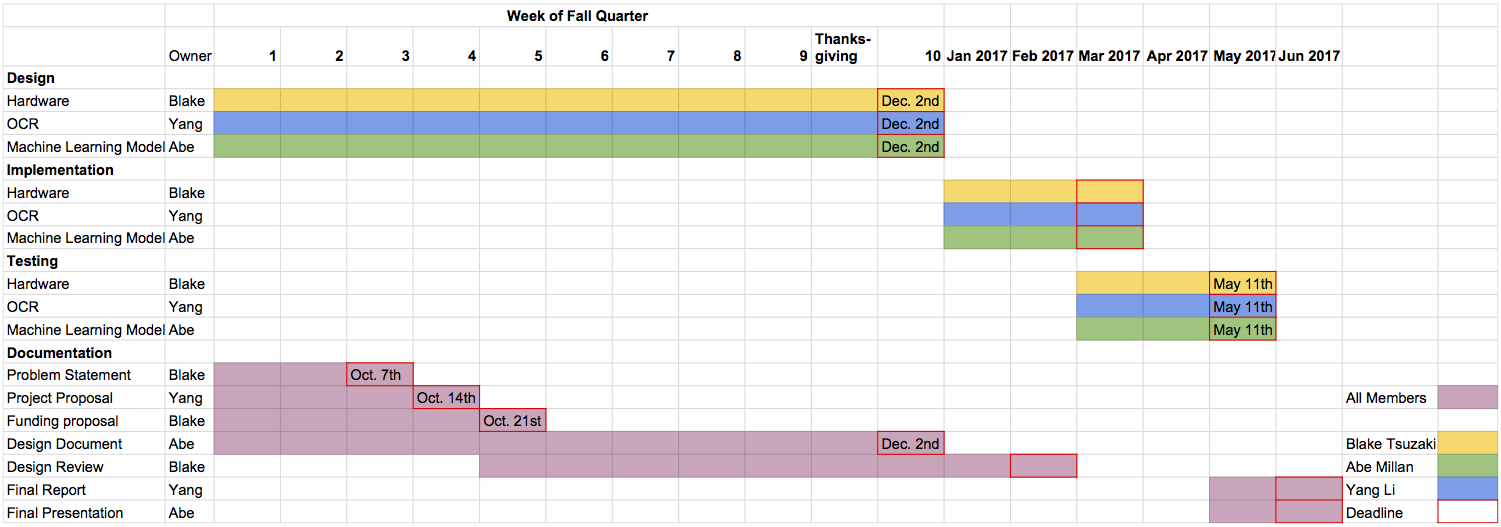
\includegraphics[angle = 90, scale = 0.8]{developmentTimeline.png}
    
    \caption{Use Cases}
\end{figure}

\backmatter
\chapter{Appendix}

\begin{figure}
	\centering
	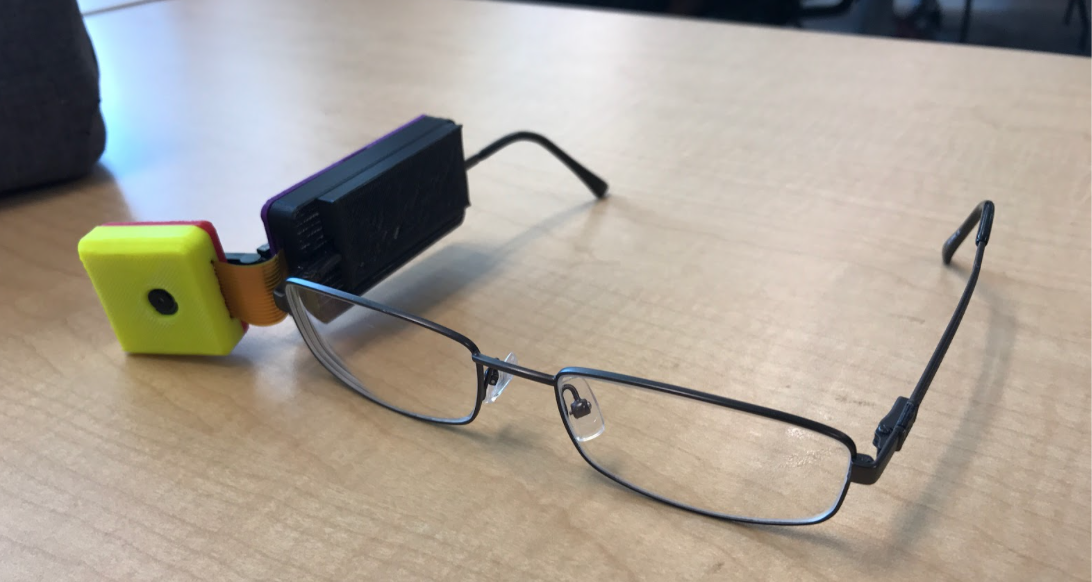
\includegraphics[scale = 0.6]{PRAHVI-HARDWARE}
	\caption{Hardware}
	\label{headsetPic}
\end{figure}

\begin{figure}
	\centering
	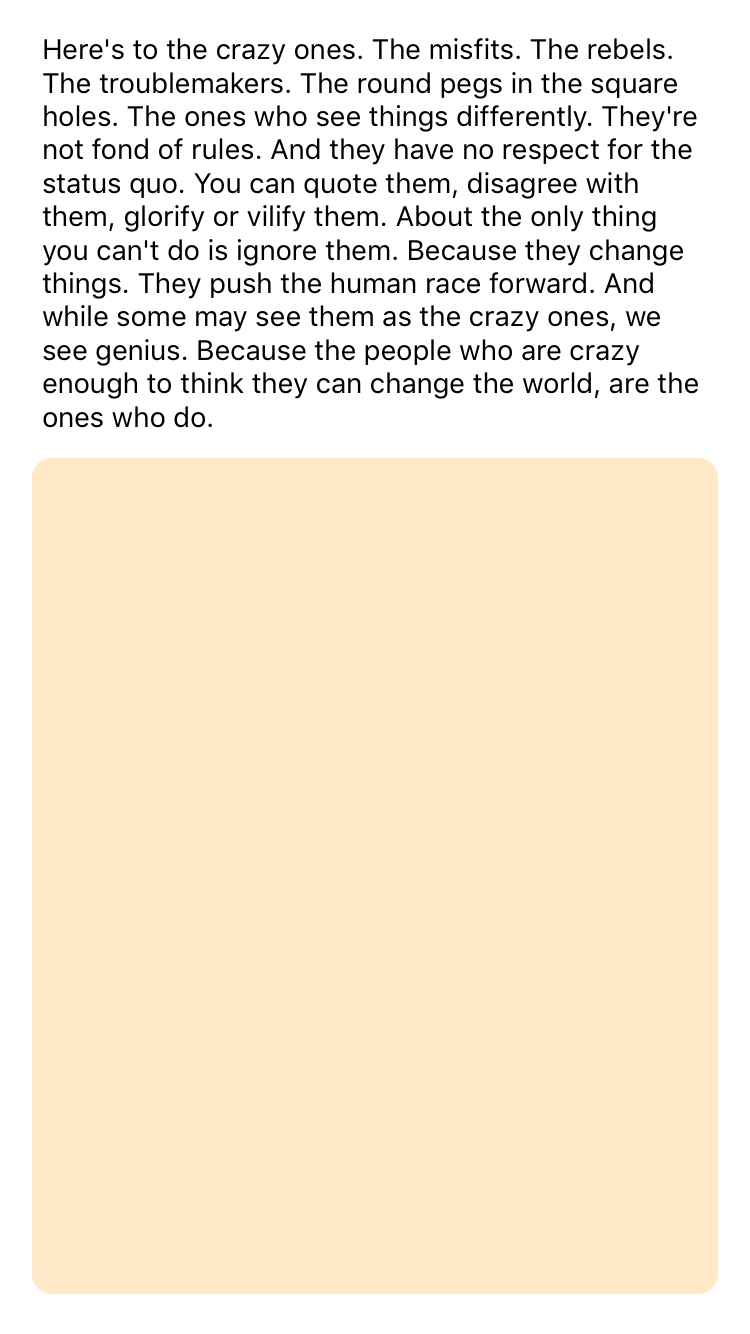
\includegraphics[scale = 0.2]{ui}
	\caption{User Interface}
	\label{uipicture}
\end{figure}

\section{Sample Testing Documents}
\subsection{Can Amazon's assistant stay on top?}
http://www.bbc.com/news/technology-39853718
\subsubsection{Original Text}
Amazon surprised everyone when, in late 2014, it unveiled a standalone digital assistant that was not only good, but blew away the competition in both quality and aesthetics.
The Echo - a cylindrical speaker with microphone - now accounts for just over 70\% of all digital assistant use in the US, leaving its nearest competitor, Google Home, well behind.
It's an important new market, even if the idea of talking to an object in your home still comes uneasily to many of us.
In a new report, Emarketer estimated 36 million Americans will use a voice-activated assistant at last once a month - an increase of 129\% on this time last year.
Amazon, as I mentioned, already has the lion's share. It's now hoping to echo (sorry) that success with its latest effort which we could see as early as Tuesday, according to reports.
AFTV.com, a site with a solid track record of leaks, said it found a low-quality image of the device on Amazon's own servers.
The authenticity of the image was later backed up by king-of-the-leaks, Evan Blass. 
The new device is expected to house a 7-inch touchscreen and can be used for video calling, as well as displaying weather information and other data.
It will help plug that gap that many voice assistant users will be familiar with, like not knowing how long a timer has left without asking. Or just knowing the time - it's a step backwards to not just look at a clock. Of course, a screen opens up a range of new possible interactions.
'Barely crossed the starting line'
Dominating this area isn't just about selling assistants. The opportunity for Amazon here is in an arena few thought they become a major player - home automation. Emarketer's data suggests that once you opt for one brand of assistant in your home, you're very unlikely to jump ship. So when the "internet of things" boom finally hits (any day now, as we've been saying the past three years) Amazon's early lead could really start to pay off.
Or, it could blow it. Consider Amazon's lead like doing well in the first event of a heptathlon.
"Amazon has a head start in the voice race but the industry has barely crossed the starting line," said CCS Insight analyst Geoff Blaber. I caught him as he was on his way to Microsoft's developer's conference, where its own digital assistant, Cortana, will be centre stage.
He added: "Those that can maximize customer data, search, artificial intelligence and natural language processing, make it all available to developers to innovate with, and simultaneously walk the privacy tightrope, will be the ultimate winners."
As it seeks to rapidly expand its lead, Amazon has made itself incredibly developer-friendly compared to its rivals. I recently had a spin in an Alexa-enabled Ford, and General Electric today announced an Alexa-powered lamp. Amazon wants Alexa in as many nooks and crannies of our lives as possible.

\subsubsection{Detected Text}
Amazon surprised everyone when. in late 2014. it unveiled a standalone diaitat assistant
that was not only good. but blew away the competition in both quality and aesthetics.
The ticho - a eytindrical speaker with microphone - now accounts for just over 70\%6 of all
Jurital ausistant use in the US, leaving its nearest competitor, Google Home, well behind.
\#'s an important new market, even if the idea of talking to an object in your home still
comes uneasity to many of us
in a new report, Emarketer estimated 36 million Americans will use a voice-activated
at last once a month - an increase of 129\% on this time last year
Amazon, as I mentioned. already has the lion's share, It's now hoping to echo (sorry) that
with its latest effort which we could see as early as Tuesday. according to reports
AIPTV.com, a site with a soild track record of leaks, said it found a low-quality image of the
device on Amazon's own servers.
The authenticity of the image was later backed up by king-of the- leaks. Evan
"The new device is expected to house a 7-inch touchscreen and can be used for video calling.
as well as displaying weather information and other data:
It will help plug that wap that many voice assistant users will be familiar with. like not
knowing how long a timer has left without asking. Or Just knowing the time -it's a step
backwards to not just look at a clack. Of course. a screen opens up a range of new possible
interactions.
"tarely croused the starting tine"
Dominating this area isn't just about selling assistants, The opportunity for Amazon here is
in an arena few thought they became a major player - home automation. Emarketer's data
sumrests that once you opt for one brand of assistant in your home. you're very unlikely to
Jurnp ship. So when the "internet of things" boom finally hits (any day nowe as we've been
saying the past three years) Amazon's early lead could really start to pay off.
Or it could blow it. Consider Amazon's lead like doing well in the first event of a heptathlon.
"Amazon has a head start in the vaice race but the industry has barely crossed the starting
line." said CCS Insight analyst Geoff caught him as he was on his way to Microsoft's
(developer's conference. where its own digital assistant, Cortana, will be centre stage:
He added: "Those that can maximize customer data, yearch, artificial intelligence and
natural language processing. make it all available to developers to innovate with. and
simultancousty walk the privacy tightrope. will be the ultimate winners."
As it seeks to rapidly expand its ead. Amazon has made itself incredibly developer-triendy
compared to its rivals I recently had 'a spin in an Alexa-enabled Ford. and General Electric
today announced an Alexa-powered lamp. Amazon wants Alexa in as many nooks and
crannies of our tives as possible.
t

\subsection{Dubai becomes first city to get its own Microsoft font}
http://www.bbc.com/news/business-39767990
\subsubsection{Original Text}
Not content with having the world's tallest building and biggest shopping centre, Dubai has become the first city to get its own Microsoft-designed font.
The typeface comes in both Latin and Arabic script, and will be available in 23 languages.
Government bodies have been told to use it in official correspondence.
But given the human rights record of Dubai and the United Arab Emirates, eyebrows will be raised at claims it is a font of "self-expression".
'Create harmony'
Dubai's Crown Prince Hamdan bin Mohammed al-Maktoum said he had been personally involved in "all the stages" of the development of the font.
It was "a very important step for us as part of our continuous efforts to be ranked first in the digital world," he added.
"We are confident that this new font and its unique specifications will prove popular among other fonts used online and in smart technologies across the world".
Dubai's government said the typeface's design "reflects modernity and is inspired by the city" and "was designed to create harmony between Latin and Arabic".
When self expression isn't usually your type
"Self-expression is an art form," says the blurb accompanying the launch of this font.
"Through it you share who you are, what you think and how you feel to the world. To do so you need a medium capable of capturing the nuances of everything you have to say.
"The Dubai Font does exactly that. It is a new global medium for self-expression."
But the United Arab Emirates - of which Dubai is part - has been criticised for its restrictions on free speech.
The constitution does guarantee the right to freedom of opinion and expression, but Human Rights Watch (HRW) says this "has no effect on the daily life of the citizen" and the country "has seen a wave of arrests and violations of human rights and freedoms and mute the voices of dissent".
In March, high-profile human rights activist Ahmed Mansoor was arrested, a move HRW said showed "complete intolerance of peaceful dissent".
The UAE's official news agency, WAM, said Mr Mansoor had been held "on suspicion of using social media sites to publish "flawed information" and "false news" to "incite sectarian strife and hatred" and "harm the reputation of the state."

\subsubsection{Detected Text}
Not content with having the world i tallest building and best shopping centre, Dubai has
become the first city to get its own Microsoft designed font:
"The typeface comes in both Latin and Arabic script. and will be available in 23 languages.
Government bodies have been told to use it in official correspondence
Wat aiven the human rights record of Dubai and the United Arab Emirates. eyebrows will be
raised at claim it in a font of "welt-expression".
'Create harmony
Bubal's Grown Prince Hamdan bin Mohammed al- Maktoum said he had been personally
involved in "all the stages" of the development of the font.
It was "a very important step for us as part of our continuous efforts to be ranked first in
the world he added.
"We are confident that this new font and its unique specifications will prove popular among
other fonts used ontine and in smart technologies across the world".
Dubai's government said the typeface's destin "reflects modernity and is inspired by the
vity" and "was destined to create harmony between Latin and Arabic'.
When self expression isn't usually your type
"Seit exnression is an art form" says the blurb accompanying the launch of this font.
"Ihrough it you share who you are. what you think and how you feel to the world. To do so
you need a medium capable of capturing the nuances of everything you have to say.
"Ime Dubai Font does exactly that. it is a new global medium for self-expression."
hat the United Arab Emirates - of which Duba is part - has been criticised for its
restrictions on tree speech
"The constitution does nuarantee the right to freedom of opinion and expression. but Human
Wights Watch (HRW) says this "has no effect on the daily life of the citizen" and the country
"has ween a wave af arrests and violations of human rights and freedoms and mute the
voices of dissent
\\n March: high profile human rights activist Ahmed Mansoor was arrested, a move HRW
said showed "compete intolerance of peaceful dissent~;
The UAE's official news agency: WAM, maid Mr Manzoor had been held "on suspicion of
using social media sites to publish "flawed information" and "false news" to "incite
sectarian strife and hatred" and "harm the reputation of the state."

\subsection{FCC website 'targeted by attack' after John Oliver comments}
http://www.bbc.com/news/technology-39855490
\subsubsection{Original Text}
The US Federal Communications Commission (FCC) website was deliberately attacked on 8 May, the regulator has said.
The incident began hours after comedian John Oliver criticised FCC plans to reverse US net neutrality rules.
Mr Oliver urged people to post to the site's online commenting system, protesting against the proposals.
The FCC said that issues with the site were caused by orchestrated attacks, not high volumes of traffic.
"These actors were not attempting to file comments themselves; rather they made it difficult for legitimate commenters to access and file with the FCC," chief information officer Dr David Bray said in an official statement.
"While the comment system remained up and running the entire time, these distributed denial of service (DDoS) events tied up the servers and prevented them from responding to people attempting to submit comments."
'Trolling the trolls'
In his Sunday night show Last Week Tonight, Mr Oliver called on viewers to visit a website that would direct them to the correct page on the FCC site to leave their comments.
"Every internet group needs to come together… gamers, YouTube celebrities, Instagram models, Tom from MySpace if you're still alive. We need all of you," he said.
His plea came after FCC chairman Ajit Pai said in April that he would review rules made in 2015 that require broadband companies to treat all online traffic equally.
Media captionEXPLAINED: What is a DDoS attack?
Last December, Mr Pai said in a speech that the net neutrality laws were "holding back investment, innovation, and job creation".
"Mr Pai is essentially trolling the trolls," Chris Marsden, professor of internet law at the University of Sussex, told the BBC.
"If you bait John Oliver, you reap what you sow."
The FCC will vote on Mr Pai's proposals to revoke the legislation on 18 May.

\subsubsection{Detected Text}
The US Fedterai Communications Commission (PCC) website was deliberately attacked on A
May: the regulator has sas
The incident began hours aer comedian John Oliver eriticised PCC plans to reverse US net
rutes
Mr Oliver urged people to post to the site's online commenting system. protesting against
the nroposais
The Fol said that issues with the ite were caused by orchestrated attacks, not high
votumes of wathic
"These actors were not attempting to file comments themselves; rather they made it
for commenters to access and fle with the PCC. chief information officer
Br David tay said in an official statement
"While the comment system remained up and running the entire time, these distributed
denial of service (DDoS)  vents tied up the servers and prevented them fram responding to
people attempting to submit comments"
"Trotting the trots
in his Sunday nught show Last Week Tonight Mr Oliver called on viewers to visit a website
that would direct them to the carrect page on the PCC site to leave their comments
"Avery internet group needs to come together... gamers. YouTube celebrities. Instagram
models Tom from MySpace if you're sul alive We need all of you" he saic.
His pes came aer FCC chairman Allt Pat sald in April that he would review rules made in
2018 Oiat require broadband companies to treat all onine traffic equally
Media captionEXPLAINED: What is a DDoS attacker
Last December. Mr Pas said in a speech that the net neutrality laws were "holding back
Investment, innovation. and job creation",
"hir Pal is eanentially trolling the trolls" Chris Marsden. professor of internet law at the
University of Sussex. told the fie.
"if you bait John Oliver. you reap what you sou"
"The FCC will vote on Mr Pais proposals to revoke the legislation on 11 May.

\pagebreak

\section{Code}
\subsection{Raspberry Pi}


\subsection{Smart Phone Application}

\subsection{Server}

\subsubsection{Text Extraction}
\begin{lstlisting}
//
//  blurDetection.cpp
//  prahvi
//
//  Created by Yang Li on 4/29/17.
//  Copyright © 2017 Portable Reading Assistant Headset for the Visually Impaired. All rights reserved.
//
//	Description: module to check whether the image (Mat object) received is blur

#include <opencv2/imgproc/imgproc.hpp>
#include "blurDetection.hpp"

//	threshold value to determine if the image is blur
#define BLUR_THRESHOLD 50

//	Function: varianceOfLaplacian
//	Description: generate the variance of Laplacian for the matrix received
double varianceOfLaplacian(cv::Mat &imageGray)
{
	cv::Mat laplacian_result;
	cv::Scalar mean;
	cv::Scalar stddev;
	
	Laplacian(imageGray, laplacian_result, CV_64F);
	meanStdDev(laplacian_result, mean, stddev);
	
	return pow((double) stddev[0],2);
}

//	Function: isBlur
//	Description: determine whether image received is blur or not
//		If the variance of Laplacian of the grayscalled image is less than the threshold
//		Then the image is blurred
bool isBlur(cv::Mat &image)
{
	cv::Mat imageGray;
	double variance;
	
	cvtColor(image, imageGray, cv::COLOR_BGR2GRAY);
	variance = varianceOfLaplacian(imageGray);
	
	if(variance < BLUR_THRESHOLD)
	{
		return true;
	}
	return false;
}
\end{lstlisting}

\begin{lstlisting}
//
//  blurDetection.hpp
//  prahvi
//
//  Created by Yang Li on 4/29/17.
//  Copyright © 2017 Portable Reading Assistant Headset for the Visually Impaired. All rights reserved.
//
//	Description: header file for blurDetection

#ifndef blurDetection_hpp
#define blurDetection_hpp

#include <opencv2/opencv.hpp>

bool isBlur(cv::Mat &image);

#endif /* blurDetection_hpp */

\end{lstlisting}

\begin{lstlisting}
//
//  getImage.cpp
//  prahvi
//
//  Created by Yang Li on 4/29/17.
//  Copyright © 2017 Portable Reading Assistant Headset for the Visually Impaired. All rights reserved.
//
//  Description: module for get the image for PRAHVI
//

#include "getImage.hpp"
#include "global.hpp"

//  Function: getImage()
//  Description: function that returns an opencv Mat object - an image for PRAHVI to process
//		Initially setup to read from a file, need to change with ios
//		TODO
cv::Mat getImage()
{
	cv::Mat image = cv::imread("/Users/Youngestyle/Desktop/image-19.jpeg");//fileAddress);
	return image;
}

\end{lstlisting}

\begin{lstlisting}
//
//  getImage.hpp
//  prahvi
//
//  Created by Yang Li on 4/29/17.
//  Copyright © 2017 Portable Reading Assistant Headset for the Visually Impaired. All rights reserved.
//
//  Description: header file for get the image for PRAHVI


#ifndef getImage_hpp
#define getImage_hpp

#include <opencv2/opencv.hpp>

cv::Mat getImage();

#endif /* getImage_hpp */

\end{lstlisting}

\begin{lstlisting}
//
//  global.hpp
//  prahvi
//
//  Created by Yang Li on 5/6/17.
//  Copyright © 2017 Portable Reading Assistant Headset for the Visually Impaired. All rights reserved.
//

#ifndef global_hpp
#define global_hpp

extern std::string fileAddress;

#endif /* global_hpp */

\end{lstlisting}

\begin{lstlisting}
//
//  imageToText.cpp
//  prahvi
//
//  Created by Yang Li on 4/29/17.
//  Copyright © 2017 Portable Reading Assistant Headset for the Visually Impaired. All rights reserved.
//
//	Description: module that converts the image received to a string of text
//		the image received is alread preprocessed
//		currently just passes the image to the google tesseract api

#include <tesseract/baseapi.h>
#include "imageToText.hpp"


//	Function: replaceString
//	Description: replace all "toReplace" with "replaceWith" in string "s"
std::string replaceString(std::string &text, const std::string &toReplace, const std::string &replaceWith)
{
	int location = 0;
	int replaceWithLength = replaceWith.length();
	
	while((location = (int) text.find(toReplace, location)) != std::string::npos)
	{
		text.replace(text.find(toReplace), toReplace.length(), replaceWith);
		location += replaceWithLength;
	}
	return text;
}

//	Function: replaceLigatures
//	Description: replace the ligatures with non-ligatures
std::string replaceLigatures(std::string text)
{
	// list of ligatures and non ligatures
	// the list is too long, and it is making the system really slow
	//std::vector<std::string> ligatures = {"Ꜳ", "ꜳ", "Æ", "æ", "Ꜵ",
	//	"ꜵ", "Ꜷ", "ꜷ", "Ꜹ", "ꜹ",
	//	"Ꜻ", "ꜻ", "Ꜽ", "ꜽ", "ff",
	//	"ffi", "ffl", "fi", "fl", "Œ",
	//	"œ", "Ꝏ", "ꝏ", "ẞ", "ß",
	//	"st", "ſt", "Ꜩ", "ꜩ", "ᵫ",
	//	"Ꝡ", "ꝡ"};
	//std::vector<std::string> nonLigatures = {"AA", "aa", "AE", "ae", "AO",
	//	"ao", "AU", "au", "AV", "av",
	//	"AV", "av", "AY", "ay", "ff",
	//	"ffi", "ffl", "fi", "fl", "OE",
	//	"oe", "OO", "oo", "fs", "fz",
	//	"st", "ft", "TZ", "tz", "ue",
	//	"VY", "vy"};
	
	// thus a shorter list of common ligatures are searched and replaced
	std::vector<std::string> ligatures = {"ff", "ffi", "ffl", "fi", "fl","st", "ſt"};
	std::vector<std::string> nonLigatures = {"ff", "ffi", "ffl", "fi", "fl", "st", "ft"};
		
	for(int i = 0; i < ligatures.size(); i++)
	{
		text = replaceString(text, ligatures[i], nonLigatures[i]);
	}
	
	return text;
}

//	Function: imageToText
//	Description: receive a Mat and pass the Mat to OCR to detect the text
//		The border of the image (Mat) is removed to reduce noise
//		The OCR is initialized for English ONLY.

std::string imageToText(cv::Mat &image)
{
	std::string outText;
	
	tesseract::TessBaseAPI *api = new tesseract::TessBaseAPI();
	
	// Initialize tesseract-ocr with English, without specifying tessdata path
	if (api->Init(NULL, "eng"))
	{
		std::cerr << "ERROR: could not initialize tesseract" << std::endl;
		exit(1);
	}
	
	// crop the image to remove the border
	// this reduces the noise from the background
	// can use fixed pixels or with respect to width and height
	
	int offsetX = image.size().width*0.05;
	int offsetY = image.size().height*0.05;
	
	cv::Rect roi;
	roi.x = offsetX;
	roi.y = offsetY;
	roi.width = image.size().width - (offsetX*2);
	roi.height = image.size().height - (offsetY*2);
	
	// crop the original image to the defined ROI
	
	image = image(roi);
	
	// send the image to OCR
	api->SetImage((uchar*)image.data,
				  image.size().width,
				  image.size().height,
				  image.channels(),
				  image.step1());
	
	// get OCR result
	api->Recognize(0);
	outText = api->GetUTF8Text();
	
	// destroy used object and release memory
	api->End();
	
	outText = replaceLigatures(outText);
	
	return outText;
}

\end{lstlisting}

\begin{lstlisting}
//
//  imageToText.hpp
//  prahvi
//
//  Created by Yang Li on 4/29/17.
//  Copyright © 2017 Portable Reading Assistant Headset for the Visually Impaired. All rights reserved.
//
//	Description: header file for imageToText

#ifndef imageToText_hpp
#define imageToText_hpp

#include <opencv2/opencv.hpp>

std::string imageToText(cv::Mat &image);

#endif /* imageToText_hpp */

\end{lstlisting}

\begin{lstlisting}
//
//  main.cpp
//  prahvi
//
//  Created by Yang Li on 4/29/17.
//  Copyright © 2017 Portable Reading Assistant Headset for the Visually Impaired. All rights reserved.
//
//	Description: the system test file after the image is received
//		this file creates the prahvi object and convert the image to text


#include <iostream>
#include "prahvi.hpp"
#include "global.hpp"

std::string fileAddress;

int main(int argc, const char * argv[]) {
	
	int result;
	std::string text;
	
	/*
	 if(argc < 2)
	{
		std::cerr << "ERROR: file name not specified" << std::endl;
		return -1;
	}
	
	fileAddress = argv[1];
	 */
	
	prahvi myPrahvi;
	text = myPrahvi.getNewText(result);
	if(result == SUCCESS)
	{
		std::cout << text << std::endl;
	}
	else if(result == EMPTY)
	{
		std::cout << "Empty image, try again" << std::endl;
	}
	
	return 0;
}

\end{lstlisting}

\begin{lstlisting}
//
//  prahvi.cpp
//  prahvi
//
//  Created by Yang Li on 4/29/17.
//  Copyright © 2017 Portable Reading Assistant Headset for the Visually Impaired. All rights reserved.
//
//  Description: prahvi class
//		the prahvi class does the preprocessing and text detection
//		other program can create and call this class to get corresponding results

#include "prahvi.hpp"
#include "getImage.hpp"
#include "blurDetection.hpp"
#include "similarityDetection.hpp"
#include "imageToText.hpp"
#include "scanner.hpp"
#include "boundingBoxDetection.hpp"

//	Function: prahvi::prahvi
//	Description: constructor for prahvi
prahvi::prahvi()
{
	_previousImage = cv::Mat::zeros(1, 1, CV_64F);
	_currentText = "";
	_currentImage = cv::Mat::zeros(1, 1, CV_64F);
}

//	Function: prahvi::getText
//	Description: get the text of the current image
std::string prahvi::getText()
{
	return _currentText;
}

//	Function: prahvi::getNewText
//	Description: get a new image and process it
//		the fucntion will get a new image
//		if the new image is blur, it will terminate
//		otherwise, it will extract the text area
//		and compare to the previous text area
std::string prahvi::getNewText(int &result)
{
	cv::Mat newImage = getImage();
	
	//	check if the new image is blurred
	if(isBlur(newImage))
	{
		result = BLUR;
		return "";
	}
	
	_previousImage = _currentImage;
	_currentImage = getTextArea(newImage);
	
	//	check if the new image is similar to the previous image
	//	TODO - uncomment after add IDF
	/*
	if(_previousImage == cv::Mat::zeros(1, 1, CV_64F) || isSimilar(_previousImage, _currentImage))
	{
		result = SIMILAR;
		return "";
	}
	 */
	
	//	convert the image to text
	_currentText = imageToText(_currentImage);
	
	//	reset TF-IDF and generate the score for the new document
	//	TODO - uncomment after add IDF
	//_tfidf.resetTerms();
	//_tfidf.addTerms(_currentText);
	
	result = EMPTY;
	
	for(int i = 0; i < _currentText.length(); i++)
	{
		if(!isspace(_currentText[i]))
		{
			result = SUCCESS;
		}
	}
	
	return _currentText;
}

std::string prahvi::getKeyword(int n)
{
	//	TODO - uncomment after add IDF
	return "";//_tfidf.getTerm(n);
}

\end{lstlisting}

\begin{lstlisting}
//
//  prahvi.hpp
//  prahvi
//
//  Created by Yang Li on 4/29/17.
//  Copyright © 2017 Portable Reading Assistant Headset for the Visually Impaired. All rights reserved.
//
//  Description: header file for prahvi class

#ifndef prahvi_hpp
#define prahvi_hpp

#include <opencv2/opencv.hpp>
#include "tfidf.hpp"

enum ProcessResult {SUCCESS, BLUR, SIMILAR, EMPTY};

class prahvi
{
public:
	prahvi();
	std::string getText();
	std::string getKeyword(int n=1);
	std::string getNewText(int &result);
	
private:
	cv::Mat _previousImage;
	cv::Mat _currentImage;
	std::string _currentText;
	//	TODO - uncomment after add IDF
	//tfidf _tfidf;
};

#endif /* prahvi_hpp */

\end{lstlisting}

\begin{lstlisting}
//
//  scanner.cpp
//  prahvi
//
//  Created by Yang Li on 4/29/17.
//  Copyright © 2017 Portable Reading Assistant Headset for the Visually Impaired. All rights reserved.
//
//	Description: module that extract the text area from the image
//		such that the result will be like a scanned document

#include <algorithm>
#include <vector>
#include "scanner.hpp"

//	Function: comaprePointSum
//	Description: compare 2 points based on the sum of the coordinate
//		return true if the first point is smaller than the second point
bool comparePointSum(cv::Point a, cv::Point b)
{
	return a.x + a.y < b.x + b.y;
}
//	Function: comaprePointDifference
//	Description: compare 2 points based on the difference of the coordinate
//		return true if the first point is smaller than the second point
bool comparePointDifference(cv::Point a, cv::Point b)
{
	return a.y - a.x < b.y - b.x;
}

//	Function: compareArea
//	Description: compare 2 points based on the contor area
//		return true if the first point is larger than the second point
bool compareArea(std::vector<cv::Point> a, std::vector<cv::Point> b)
{
	return contourArea(a) > contourArea(b);
}

//	Function: getDistance
//	Description: return the distance between two points
int getDistance(cv::Point a, cv::Point b)
{
	return sqrt(pow((double)b.x - (double)a.x, 2) + pow((double)b.y - (double)a.y, 2));
}

//	Function: sortContours
//	Description: sort the contours based on the contour area
//		in descending order
void sortContours(std::vector<std::vector<cv::Point>> &contours)
{
	sort(contours.begin(), contours.end(), compareArea);
}

//	Function: getTextArea
//	Description: extract the text area from the image
//		Based on find the largest contour with 4 sides in the image
//		this function also transform the result found and rectify it
cv::Mat getTextArea(cv::Mat &image)
{
	// convert to grayscale and blur
	image.convertTo(image, -1, 1, 20);
	cv::Mat imageGray;
	cvtColor(image, imageGray, CV_BGR2GRAY);
	
	cv::Mat blurred;
	GaussianBlur(imageGray, blurred, cv::Size(5, 5), 0);
	
	// apply Canny Edge Detection to find the edges
	cv::Mat edged;
	Canny(blurred, edged, 0, 50);
	
	//	find the contours in the edged image
	std::vector<std::vector<cv::Point>> contours;
	std::vector<cv::Vec4i> hierarchy;
	
	findContours(edged, contours, hierarchy, cv::RETR_LIST, cv::CHAIN_APPROX_NONE);
	
	//	sort the contours in descending order
	sortContours(contours);
	
	//	initialize the screen contour
	std::vector<cv::Point> screenContour;
	std::vector<cv::Point> approx;
	
	//	set screen contour to the largest contour with 4 sides
	for(int i = 0; i < contours.size(); i++)
	{
		double peri = arcLength(contours[i], true);
		
		approxPolyDP(cv::Mat(contours[i]), approx, 0.02*peri,true);
		
		if(approx.size() == 4)
		{
			screenContour = approx;
			break;
		}
	}
	
	std::vector<std::vector<cv::Point>> screen;
	screen.push_back(screenContour);
	
	//	initialize transformation
	cv::Mat lambda(2, 4, CV_32FC1);
	lambda = cv::Mat::zeros(image.rows, image.cols, image.type());
	
	//	input and output coordinates
	cv::Point2f inputQuad[4];
	cv::Point2f outputQuad[4];
	
	//	find the max dimension of the crop
	cv::Point topLeft, topRight, bottomRight, bottomLeft;
	
	//	the top left point has the smallest sum
	topLeft = *min_element(screenContour.begin(), screenContour.end(), comparePointSum);
	
	//	the bottom right point has the largest sum
	bottomRight = *max_element(screenContour.begin(), screenContour.end(), comparePointSum);
	
	//	the top right point has the smallest difference
	topRight = *min_element(screenContour.begin(), screenContour.end(), comparePointDifference);
	
	//	the bottom left point has the largest difference
	bottomLeft = *max_element(screenContour.begin(), screenContour.end(), comparePointDifference);

	//	set input coordinates
	inputQuad[0] = topLeft;
	inputQuad[1] = topRight;
	inputQuad[2] = bottomRight;
	inputQuad[3] = bottomLeft;
	
	//	the dimension of the output is based on the input
	//	1:1 ratio
	int width = std::max(getDistance(topLeft, topRight), getDistance(bottomLeft, bottomRight));
	int height = std::max(getDistance(topLeft, bottomLeft), getDistance(topRight, bottomRight));
	
	//	the output coordinates is based on the output dimention
	outputQuad[0] = cv::Point2f(0,0);
	outputQuad[1] = cv::Point2f(width-1, 0);
	outputQuad[2] = cv::Point2f(width-1, height-1);
	outputQuad[3] = cv::Point2f(0, height-1);
	
	//	set up transformation
	lambda = getPerspectiveTransform(inputQuad, outputQuad);
	
	cv::Mat output;
	
	//	apply transformation
	warpPerspective(image, output, lambda, cv::Size(width,height));
	
	return output;
}

\end{lstlisting}

\begin{lstlisting}
//
//  scanner.hpp
//  prahvi
//
//  Created by Yang Li on 4/29/17.
//  Copyright © 2017 Portable Reading Assistant Headset for the Visually Impaired. All rights reserved.
//
//	Description: header file for the scanner module

#ifndef scanner_hpp
#define scanner_hpp

#include <opencv2/opencv.hpp>

cv::Mat getTextArea(cv::Mat &image);

#endif /* scanner_hpp */

\end{lstlisting}

\begin{lstlisting}
//
//  similarityDetection.cpp
//  prahvi
//
//  Created by Yang Li on 4/29/17.
//  Copyright © 2017 Portable Reading Assistant Headset for the Visually Impaired. All rights reserved.
//
//	Description: module to detect whether the two image received are similar
//		Currently, the method used is AKAZE tracking
//		Can be improved using matching



#include <opencv2/features2d.hpp>
#include <opencv2/imgcodecs.hpp>
#include <vector>
#include "similarityDetection.hpp"

//	threshold value to determine whether the two images are similar
#define FEATURE_THRESHOLD 1000


const float inlier_threshold = 2.5f; // Distance threshold to identify inliers
const float nn_match_ratio = 0.8f;   // Nearest neighbor matching ratio

//	Function: akazeTracking
//	Description: comapre two images and return the number of good match points
//		Uses the A-Kaze tracking
int akazeTracking(cv::Mat &image1, cv::Mat &image2)
{
	// convert the images to grayscale
	cv::Mat image1Gray;
	cv::Mat image2Gray;
	
	cvtColor(image1, image1Gray, cv::COLOR_BGR2GRAY);
	cvtColor(image2, image2Gray, cv::COLOR_BGR2GRAY);
	
	
	// detect keypoints and compute descriptors using A-KAZE
	std::vector<cv::KeyPoint> keyPoints1, keyPoints2;
	cv::Mat descriptors1, descriptors2;
	
	cv::Ptr<cv::AKAZE> akaze = cv::AKAZE::create();
	akaze->detectAndCompute(image1Gray, cv::noArray(), keyPoints1, descriptors1);
	akaze->detectAndCompute(image2Gray, cv::noArray(), keyPoints2, descriptors2);
	
	// use the brute force matcher to find 2-nn matches
	cv::BFMatcher matcher(cv::NORM_HAMMING);
	std::vector<std::vector<cv::DMatch>> nn_matches;
	matcher.knnMatch(descriptors1, descriptors2, nn_matches, 2);
	
	// if one or more of the image does not have any keypoint, return 0
	if(keyPoints1.size() <= 0 || keyPoints2.size() <= 0)
	{
		return 0;
	}
	
	// use 2-nn matches to find correct keypoint matches
	std::vector<cv::KeyPoint> matched1, matched2, inliers1, inliers2;
	std::vector<cv::DMatch> good_matches;
	
	for(size_t i = 0; i < nn_matches.size(); i++)
	{
		cv::DMatch first = nn_matches[i][0];
		
		float distance1 = nn_matches[i][0].distance;
		float distance2 = nn_matches[i][1].distance;
		
		if(distance1 < nn_match_ratio * distance2)
		{
			matched1.push_back(keyPoints1[first.queryIdx]);
			matched2.push_back(keyPoints2[first.trainIdx]);
		}
	}
	
	// check if the matches is within the inlier_threshold
	for(unsigned i = 0; i < matched1.size(); i++) {
		cv::Mat col = cv::Mat::ones(3, 1, CV_64F);
		col.at<double>(0) = matched1[i].pt.x;
		col.at<double>(1) = matched1[i].pt.y;
		
		col /= col.at<double>(2);
		double distance = sqrt(
						   pow(col.at<double>(0) - matched2[i].pt.x, 2)
						   + pow(col.at<double>(1) - matched2[i].pt.y, 2)
						   );
		
		if(distance < inlier_threshold) {
			int new_i = static_cast<int>(inliers1.size());
			inliers1.push_back(matched1[i]);
			inliers2.push_back(matched2[i]);
			good_matches.push_back(cv::DMatch(new_i, new_i, 0));
		}
	}
	return good_matches.size();
}

bool isSimilar(cv::Mat &image1, cv::Mat &image2)
{
	if(akazeTracking(image1, image2) > FEATURE_THRESHOLD)
	{
		return true;
	}
	return false;
}

\end{lstlisting}

\begin{lstlisting}
//
//  similarityDetection.hpp
//  prahvi
//
//  Created by Yang Li on 4/29/17.
//  Copyright © 2017 Portable Reading Assistant Headset for the Visually Impaired. All rights reserved.
//
//	Description: header file for similarityDetection

#ifndef similarityDetection_hpp
#define similarityDetection_hpp

#include <opencv2/opencv.hpp>
bool isSimilar(cv::Mat &img1, cv::Mat &img2);

#endif /* similarityDetection_hpp */

\end{lstlisting}


\begin{lstlisting}

\end{lstlisting}




\begin{thebibliography}{1}

	\bibitem{PechPacheco} Pech-Pacheco, José Luis, et al. "Diatom autofocusing in brightfield microscopy: a comparative study." {\em Pattern Recognition, 2000. Proceedings. 15th International Conference on}. Vol. 3. IEEE, 2000

	\bibitem{akaze} "AKAZE local features matching." {\em AKAZE local features matching — OpenCV 3.0.0-dev documentation}. N.p., n.d. Web. 14 June 2017.
	\textless http://docs.opencv.org/3.0-beta/doc/tutorials/features2d/akaze\_matching/akaze\_matching.html\textgreater.

	\bibitem{gaussianBlur} "Image Filtering." {\em Image Filtering — OpenCV 2.4.13.2 documentation}. N.p., n.d. Web. 14 June 2017.
	\textless http://docs.opencv.org/2.4/modules/imgproc/doc/filtering.html?highlight=gaussianblur\#gaussianblur\textgreater.

	\bibitem{canny} "Canny Edge Detector." {\em Canny Edge Detector — OpenCV 2.4.13.2 documentation}. N.p., n.d. Web. 14 June 2017.
	\textless http://docs.opencv.org/2.4/doc/tutorials/imgproc/imgtrans/canny\_detector/canny\_detector.html\textgreater.

	\bibitem{contours} "Structural Analysis and Shape Descriptors." {\em Structural Analysis and Shape Descriptors — OpenCV 2.4.13.2 documentation}. N.p., n.d. Web. 14 June 2017.
	\textless http://docs.opencv.org/2.4/modules/imgproc/doc/structural\_analysis\_and\_shape\_descriptors.html?
	highlight=findcontours\#findcontours\textgreater.

	\bibitem{tfidf} "Tf-idf :: A Single-Page Tutorial - Information Retrieval and Text Mining." {\em Tf-idf :: A Single-Page Tutorial - Information Retrieval and Text Mining}. N.p., n.d. Web. 14 June 2017.
	\textless http://www.tfidf.com/\textgreater.

	\bibitem{tesseract3} Tesseract-ocr. "Tesseract-ocr/tesseract." {\em GitHub}. N.p., n.d. Web. 14 June 2017.
	\textless https://github.com/tesseract-ocr/tesseract/wiki\textgreater.
	
	\bibitem{tesseract4} Tesseract-ocr. "Tesseract-ocr/tesseract." {\em GitHub}. N.p., n.d. Web. 14 June 2017.
	\textless https://github.com/tesseract-ocr/tesseract/wiki/4.0-with-LSTM\textgreater.

\end{thebibliography}
\end{document}
